\documentclass[10pt,twocolumn]{article}

% ── Packages ──────────────────────────────────────────────────────────────────
\usepackage[margin=1in,top=1.1in,bottom=1.1in]{geometry}
\usepackage{amsmath,amssymb}
\usepackage{graphicx}
\usepackage{booktabs}
\usepackage{caption}
\usepackage{subcaption}
\usepackage{hyperref}
\usepackage{xcolor}
\usepackage{enumitem}
\usepackage{microtype}
\usepackage{float}
\usepackage{array}

\captionsetup{font=small, labelfont=bf}
\hypersetup{colorlinks=true, linkcolor=blue, citecolor=blue, urlcolor=blue}

% ── Title ─────────────────────────────────────────────────────────────────────
\title{\textbf{Medical Image Reconstruction from Edge Features:\\
Evaluating Standard and Sparsely Supervised Training\\
across Imaging Modalities}}

\author{medRecon}
\date{}

% ──────────────────────────────────────────────────────────────────────────────
\begin{document}
\maketitle

% ── Abstract ──────────────────────────────────────────────────────────────────
\begin{abstract}
We study whether a ResNet34-backed U-Net can reconstruct grayscale medical images
from three complementary edge-feature maps---Canny binary edges, Sobel gradient
magnitude, and Laplacian second derivatives---and whether sparsely supervising
only a random subset of output pixels during training improves generalisation.
We train one model per modality (chest X-ray, chest CT, brain MRI) under two
regimes: (1)~a standard pixel-wise $\ell_1$ baseline, and (2)~a Bernoulli-masked
sparse loss that omits 80\% of pixel gradients per iteration, adapted from the
Sparsely Supervised Diffusion (SSD) strategy of \cite{ssd2025}.
On all three modalities the pretrained U-Net learns to reconstruct global anatomy
from edge features within 50 epochs.
CT yields the highest reconstruction quality (PSNR 29.0\,dB, SSIM 0.854),
followed by X-ray (24.5\,dB, 0.849) and MRI (19.6\,dB, 0.616).
Sparse supervision provides no benefit: the SSD variant loses up to 0.9\,dB on
X-ray and CT and has negligible effect on MRI, indicating that an
ImageNet-pretrained encoder trained on 500 images does not exhibit the
memorisation pathology that SSD is designed to correct.
\end{abstract}

% ── 1. Introduction ───────────────────────────────────────────────────────────
\section{Introduction}
\label{sec:intro}

Medical image acquisition is expensive and modality-specific.
Edge maps---compact structural summaries that highlight intensity discontinuities
in an image---are cheap to compute and modality-agnostic.
A model that can faithfully reconstruct the original image from its edge
representation could underpin downstream tasks such as compression, modality
transfer, or anatomy segmentation without access to the full raw scan.

This work explores that setting across three clinically relevant imaging
modalities: chest X-ray, chest CT, and brain MRI.
We extract a three-channel edge feature representation from each grayscale image
using classical operators (Canny, Sobel, Laplacian), then train an encoder--decoder
network to invert the representation back to the original image.

In addition to a fully supervised baseline, we evaluate a sparsely supervised
training variant inspired by the Sparsely Supervised Diffusion (SSD) framework
\cite{ssd2025}, which proposes that randomly masking a large fraction of pixel
gradients during training forces generative models to rely on global context
rather than memorising local texture.
We ask whether this inductive bias is also beneficial for a deterministic
regression network operating on edge inputs.

% ── 2. Data ───────────────────────────────────────────────────────────────────
\section{Data}
\label{sec:data}

\subsection{Datasets}

Three publicly available Kaggle datasets are used, one per imaging modality.

\textbf{X-ray} --- COVID-19 Radiography Database \cite{xray_data}.
Posteroanterior chest radiographs organised into three diagnostic categories
(COVID-19, Normal, and Lung Opacity). Images are stored as PNG files within
per-class subdirectories.

\textbf{CT} --- Chest CT Scan Images \cite{ct_data}.
Axial chest CT slices provided in pre-split \texttt{train} and \texttt{valid}
subdirectories. Images are in PNG format.

\textbf{MRI} --- Brain MRI Images for Brain Tumor Detection \cite{mri_data}.
Coronal/axial brain MRI scans organised into two folders indicating the presence
or absence of a tumour. Images are JPEG files.

\subsection{Splits and Preprocessing}

All images are loaded as grayscale, resized to $256\times 256$ pixels with
bilinear interpolation, and normalised to $[0, 1]$ as 32-bit floats.
For each modality, images are shuffled with a fixed seed, and the first 500 are
used for training and the next 100 for validation.
No label information (diagnosis class) is used during training; the network
learns image reconstruction only.

\begin{table}[h]
\centering
\caption{Dataset summary.}
\label{tab:datasets}
\small
\begin{tabular}{lccc}
\toprule
Modality & Train & Val & Resolution \\
\midrule
X-ray (Chest)  & 500 & 100 & $256\times256$ \\
CT (Chest)     & 500 & 100 & $256\times256$ \\
MRI (Brain)    & 500 & 100 & $256\times256$ \\
\bottomrule
\end{tabular}
\end{table}

% ── 3. Method ─────────────────────────────────────────────────────────────────
\section{Method}
\label{sec:method}

\subsection{Input Transforms: Edge Feature Extraction}
\label{sec:transforms}

Given a normalised grayscale image $I \in [0,1]^{H \times W}$, three
complementary edge representations are computed and stacked into a
three-channel tensor $\mathbf{x} \in [0,1]^{3 \times H \times W}$ that serves
as the network input.
The ground-truth target $y \in [0,1]^{1 \times H \times W}$ is the original
image itself.

\subsubsection*{Channel 1 --- Canny Binary Edges}

The Canny detector \cite{canny1986} applies Gaussian smoothing followed by
non-maximum suppression and hysteresis thresholding to produce a thin binary
edge map:

\begin{equation}
  x_{\text{Canny}}(i,j) = \frac{1}{255}\,\text{Canny}\!\left(I;\,T_{\ell}=50,\,T_{h}=150\right)(i,j)
  \label{eq:canny}
\end{equation}

where $T_{\ell}$ and $T_h$ are the low and high hysteresis thresholds.
A pixel is retained as an edge only if its gradient magnitude exceeds $T_h$, or
if it lies between $T_{\ell}$ and $T_h$ and is 8-connected to a strong edge.

\subsubsection*{Channel 2 --- Sobel Gradient Magnitude}

The Sobel operator estimates first-order partial derivatives with a $3\times3$
kernel, and the gradient magnitude is clipped to $[0,1]$:

\begin{equation}
  x_{\text{Sobel}}(i,j) = \min\!\left(\sqrt{(K_x * I)^2 + (K_y * I)^2},\; 1\right)
  \label{eq:sobel}
\end{equation}

where $*$ denotes convolution and

\[
  K_x = \begin{bmatrix} -1 & 0 & 1 \\ -2 & 0 & 2 \\ -1 & 0 & 1 \end{bmatrix},
  \quad
  K_y = \begin{bmatrix} 1 & 2 & 1 \\ 0 & 0 & 0 \\ -1 & -2 & -1 \end{bmatrix}.
\]

Unlike Canny, the Sobel map is a soft (continuous) edge representation that
encodes gradient strength rather than binary presence.

\subsubsection*{Channel 3 --- Laplacian (Second Derivative)}

The Laplacian of the image highlights regions of rapid intensity change by
computing a discrete approximation to $\nabla^2 I$:

\begin{equation}
  x_{\text{Lap}}(i,j) = \min\!\left(\bigl|\nabla^2 I(i,j)\bigr|,\; 1\right)
  \label{eq:laplacian}
\end{equation}

where $\nabla^2$ is approximated by a $3\times3$ kernel with coefficient
$-4$ at the centre.
Taking the absolute value and clipping provides a non-negative feature map
complementary to the gradient-based Sobel channel.

\subsubsection*{Combined Input}

The three channels are stacked:

\begin{equation}
  \mathbf{x} = \bigl[x_{\text{Canny}},\; x_{\text{Sobel}},\; x_{\text{Lap}}\bigr]
  \;\in\; [0,1]^{3\times H\times W}
  \label{eq:input}
\end{equation}

This representation captures binary structure (Canny), gradient strength
(Sobel), and curvature (Laplacian) simultaneously.
No further data augmentation is applied; features are computed deterministically.

\subsection{Model Architecture: ResNet34 U-Net}
\label{sec:model}

The network is a U-Net \cite{unet2015} with a ResNet34 \cite{he2016}
encoder pre-trained on ImageNet \cite{imagenet2009}, instantiated via the
\texttt{segmentation\_models\_pytorch} library.

\begin{figure*}[t]
  \centering
  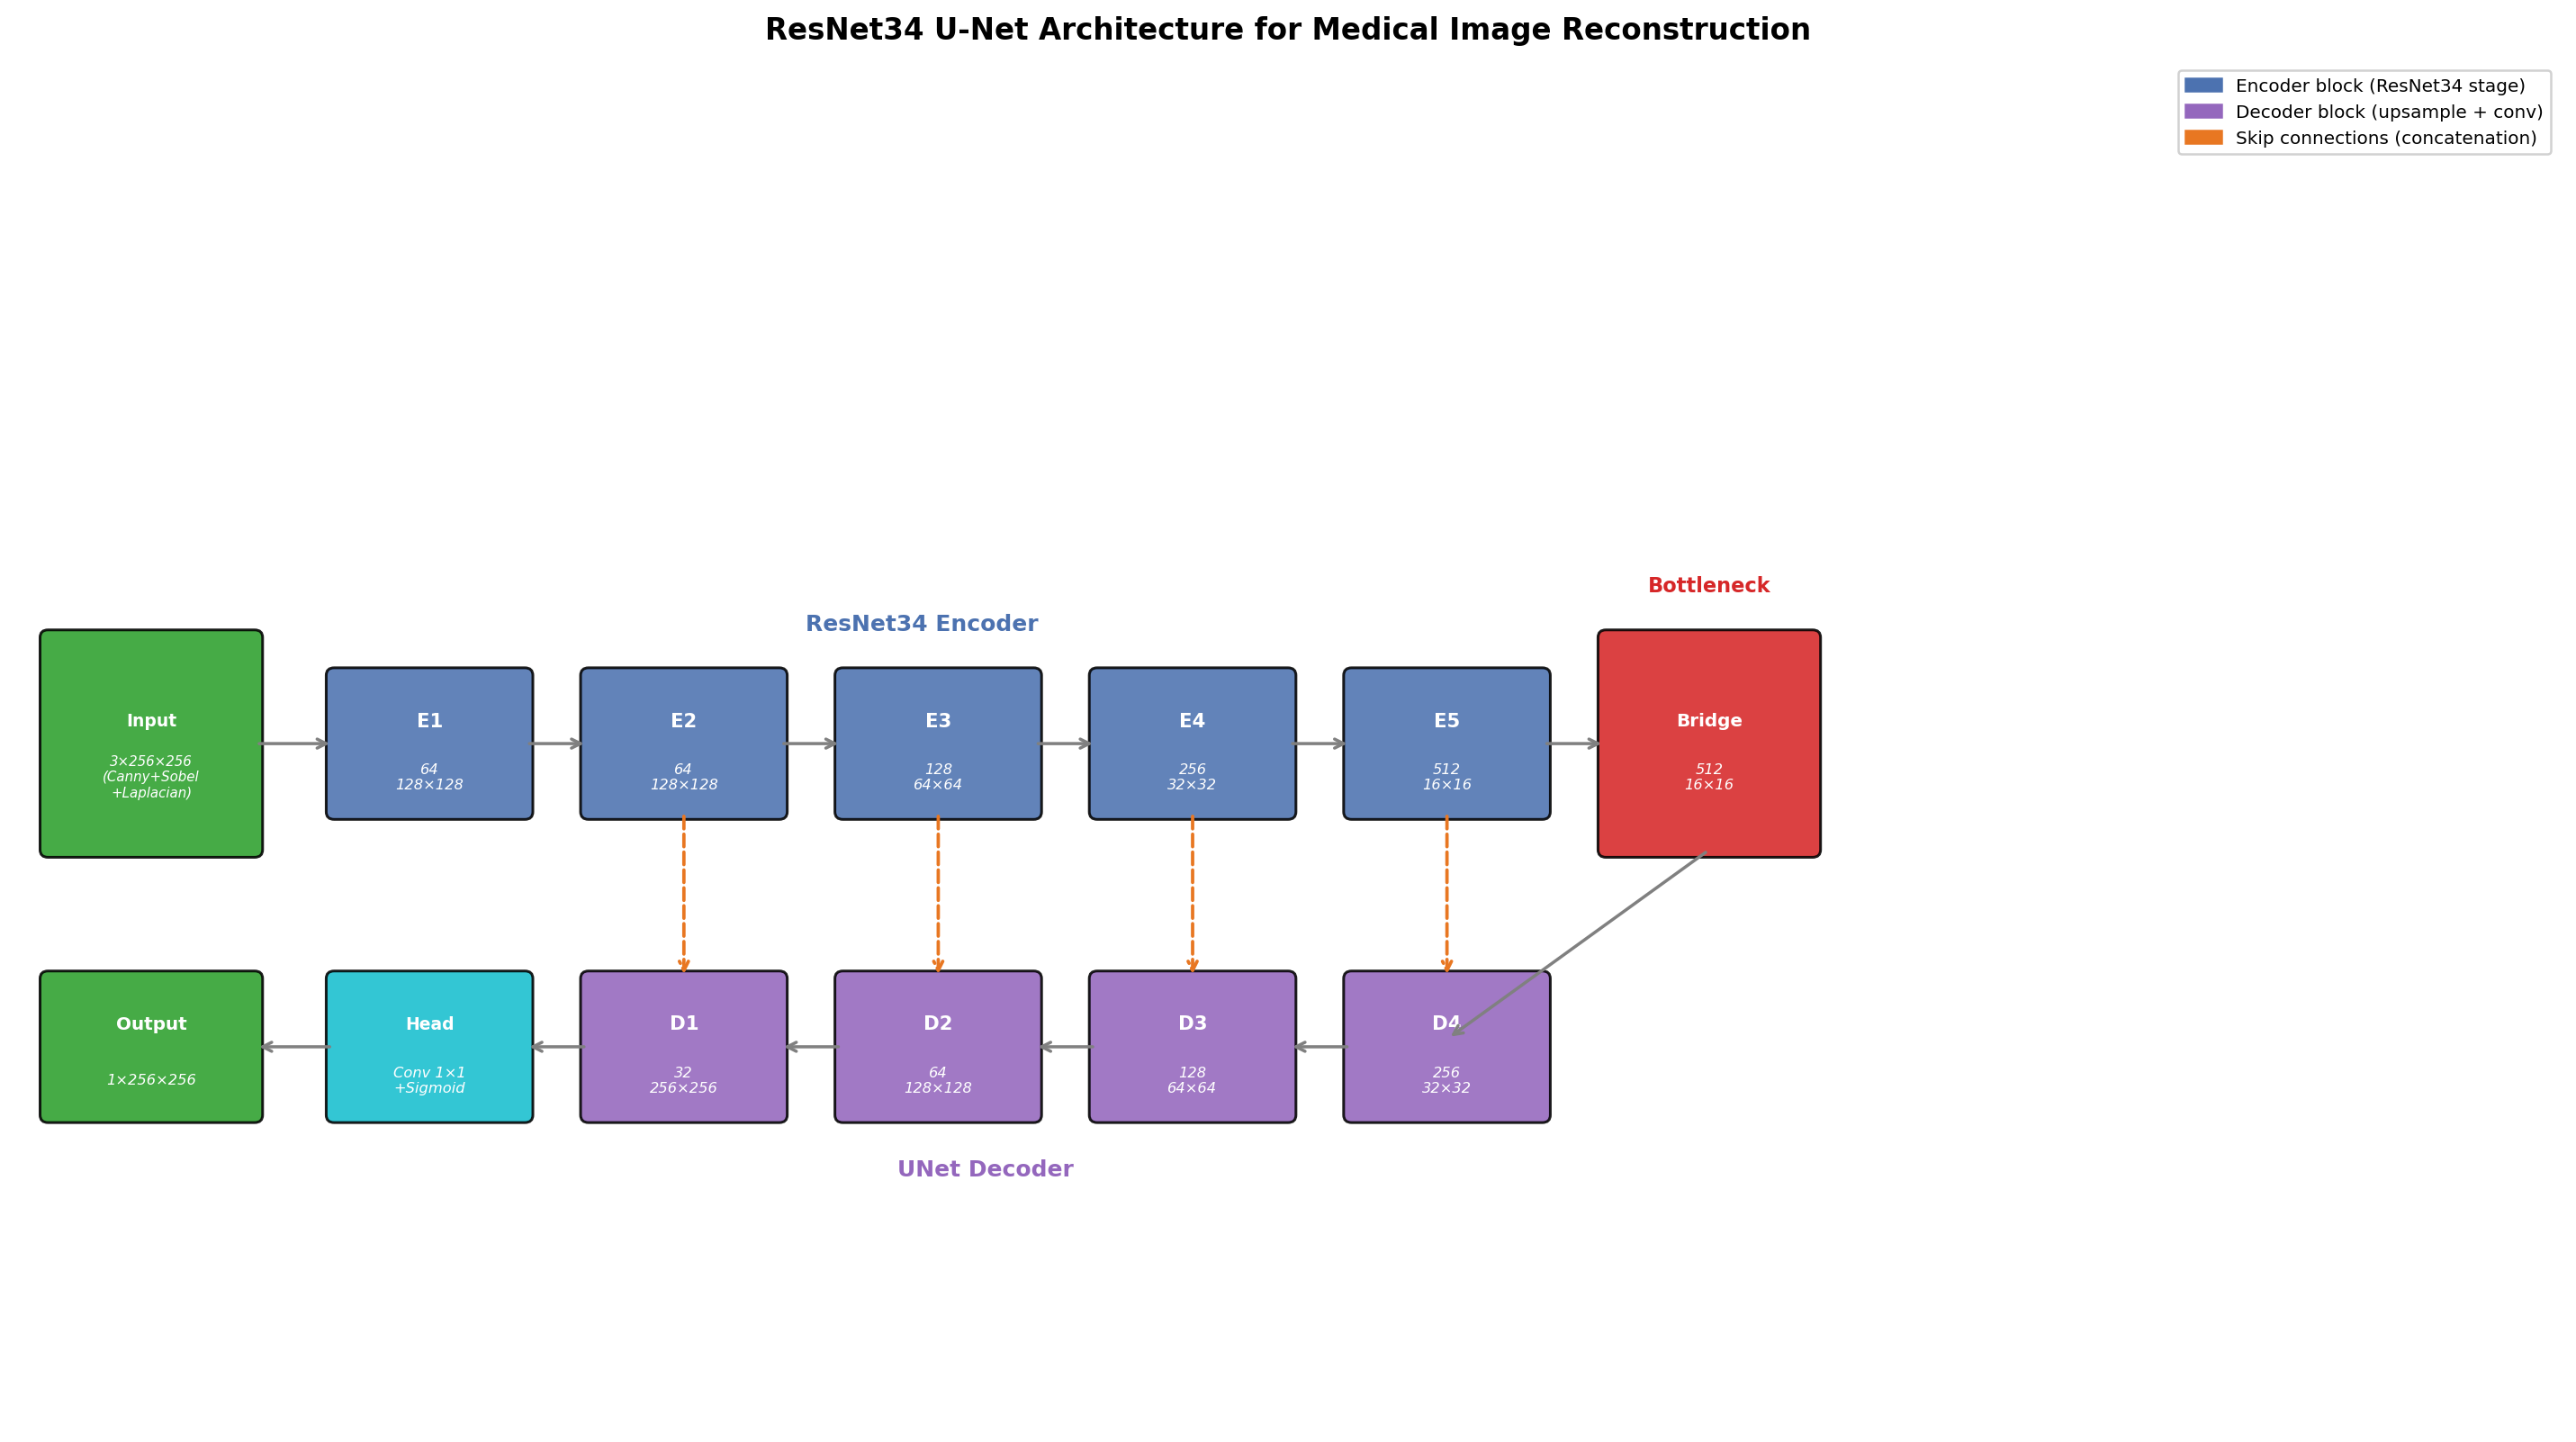
\includegraphics[width=\textwidth]{figures/unet_architecture.png}
  \caption{%
    ResNet34 U-Net architecture used in both experiments.
    The encoder (blue) extracts feature maps at five spatial scales via the
    five stages of ResNet34.
    Orange dashed arrows denote skip connections that concatenate encoder
    feature maps into the corresponding decoder stage.
    The bottleneck (red) holds the coarsest representation (512 channels,
    $16\times16$).
    The decoder (purple) progressively up-samples back to the input resolution.
    A final $1\times1$ convolution followed by a sigmoid activation produces
    the single-channel reconstruction in $[0,1]$.%
  }
  \label{fig:arch}
\end{figure*}

\textbf{Encoder.}
ResNet34 is organised into an initial strided convolution block followed by
four residual stages.
Beginning from the $256\times256$ input, the encoder produces feature maps at
decreasing spatial resolutions ($128^2$, $64^2$, $32^2$, $16^2$) with
increasing channel depths (64, 128, 256, 512).
Residual connections within each stage ease gradient flow during fine-tuning.

\textbf{Bottleneck.}
The coarsest feature map ($512 \times 16 \times 16$) is passed through the
bottleneck, which serves as the global representation from which the decoder
must recover fine-grained intensity detail.

\textbf{Decoder.}
Four decoder blocks progressively restore the spatial resolution.
Each block up-samples by a factor of two (bilinear interpolation followed by
convolution), then concatenates the corresponding encoder skip connection,
and applies two $3\times3$ convolutional layers with batch normalisation and ReLU.

\textbf{Output head.}
A $1\times1$ convolution reduces the final 32-channel feature map to a
single channel, followed by a sigmoid activation, yielding the reconstructed
image $\hat{y} \in [0,1]^{1\times256\times256}$.

The architecture is shared across all modalities; a separate model instance is
trained per modality per experiment.

% ── 4. Training ───────────────────────────────────────────────────────────────
\section{Training}
\label{sec:training}

\subsection{Common Setup}

All experiments use the Adam optimiser \cite{adam2014} with learning rate
$10^{-3}$ and default momentum parameters.
Models are trained for 50 epochs with a batch size of 16.
At each epoch the model is evaluated on the held-out validation split; the
checkpoint with the lowest validation loss is retained.
Metrics are logged per epoch for later analysis.

\subsection{Experiment 1 --- Baseline: Pixel-Wise $\ell_1$ Loss}
\label{sec:baseline}

The baseline trains each model with the standard mean absolute error over
all output pixels:

\begin{equation}
  \mathcal{L}_{\text{base}} = \frac{1}{|\Omega|}
    \sum_{(i,j)\in\Omega} \bigl|\hat{y}(i,j) - y(i,j)\bigr|
  \label{eq:l1}
\end{equation}

where $\Omega$ is the set of all $H\times W$ pixel locations and $|\Omega|$
is its cardinality.
$\ell_1$ is preferred over $\ell_2$ for image regression because it is less
sensitive to outlier intensities and tends to produce sharper reconstructions.

\subsection{Experiment 2 --- Sparsely Supervised Diffusion (SSD) Loss}
\label{sec:ssd}

\subsubsection*{Motivation}

The SSD loss is adapted from \cite{ssd2025}, where it is proposed to address
\emph{memorisation} in generative diffusion models trained on small datasets:
when a model has enough capacity to memorise training images, it fails to
generalise to unseen samples.
The proposed remedy is to supervise the model on only a random sparse subset
of pixels per iteration, forcing it to reason about global context to
hallucinate the unobserved pixels correctly.
We investigate whether this inductive bias also benefits a deterministic
regression network trained on edge features.

\subsubsection*{Formulation}

A binary mask $M \in \{0, 1\}^{H\times W}$ is drawn independently per
pixel from a Bernoulli distribution:

\begin{equation}
  M(i,j) \;\sim\; \text{Bernoulli}(1 - \eta)
  \label{eq:mask}
\end{equation}

where $\eta \in [0,1)$ is the \emph{masking ratio}.
Pixels with $M(i,j)=0$ are masked out; only the unmasked fraction
$(1-\eta)$ contributes to the loss:

\begin{equation}
  \mathcal{L}_{\text{SSD}} =
    \frac{\displaystyle\sum_{(i,j)\in\Omega}
          \bigl|\hat{y}(i,j) - y(i,j)\bigr|\cdot M(i,j)}
         {\displaystyle\sum_{(i,j)\in\Omega} M(i,j) + \varepsilon}
  \label{eq:ssd}
\end{equation}

with $\varepsilon = 10^{-8}$ for numerical stability.
A new mask is sampled at every training step, so every mini-batch sees a
different random supervision pattern.
At $\eta = 0$, equation~\eqref{eq:ssd} reduces to
equation~\eqref{eq:l1}.
The validation loss is computed using the same formula with the configured
$\eta$, ensuring consistent model selection.

\begin{figure}[h]
  \centering
  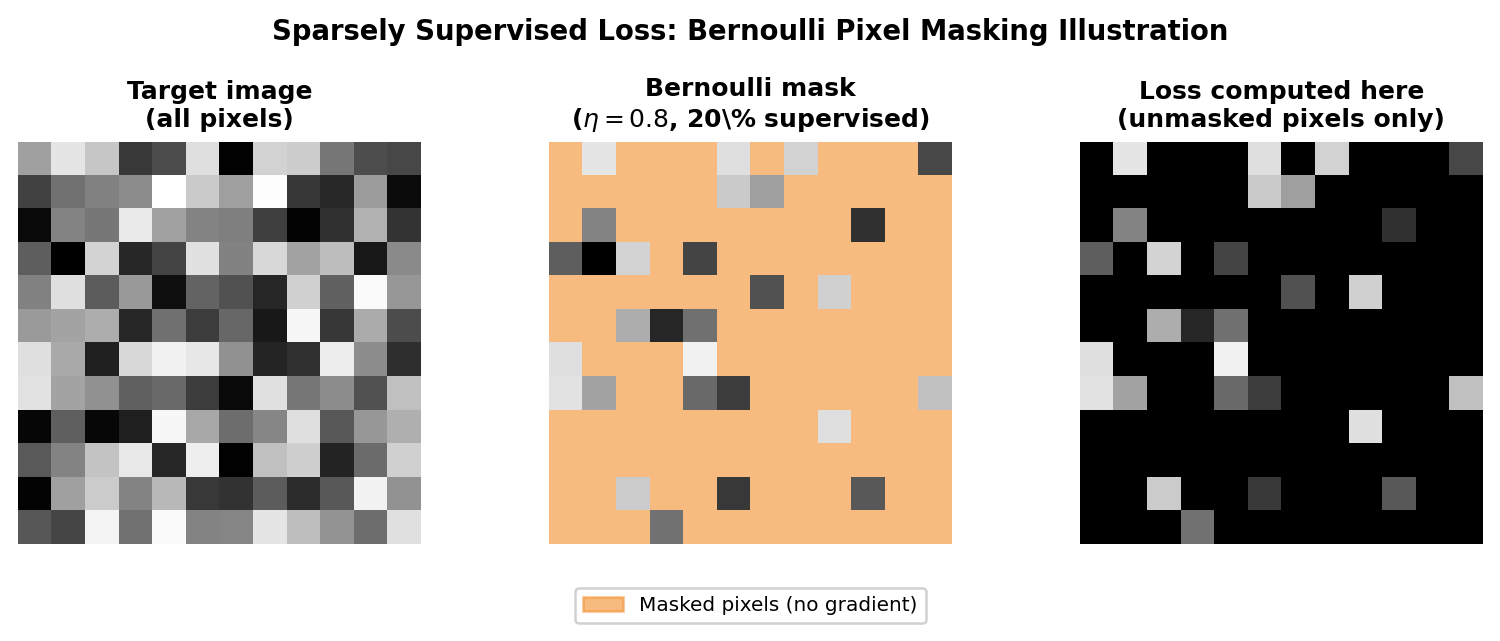
\includegraphics[width=\columnwidth]{figures/ssd_masking.png}
  \caption{%
    Illustration of Bernoulli pixel masking at $\eta=0.8$.
    Orange pixels in the middle panel are masked out; the rightmost panel
    shows the only pixels that contribute to the SSD loss.
    A fresh mask is sampled every training step.%
  }
  \label{fig:ssd_mask}
\end{figure}

We evaluate the SSD variant with masking ratio $\eta = 0.8$, meaning the model
is supervised on only 20\% of pixels per iteration.
The same ResNet34 U-Net architecture, optimiser, and dataset splits are used as
in the baseline; the only change is the loss function.

% ── 5. Results ────────────────────────────────────────────────────────────────
\section{Results}
\label{sec:results}

All models are evaluated on the held-out validation split using three metrics:
Peak Signal-to-Noise Ratio (PSNR, in dB), Structural Similarity Index (SSIM),
and Mean Absolute Error (MAE).
Higher PSNR and SSIM indicate better reconstruction; lower MAE indicates smaller
pixel-level error.

\subsection{Baseline Results}

Table~\ref{tab:baseline} reports final-epoch metrics for the three modality-specific
baseline models.

\begin{table}[h]
\centering
\caption{Baseline ($\eta=0$) validation metrics at epoch 50.}
\label{tab:baseline}
\small
\begin{tabular}{lcccc}
\toprule
Modality & PSNR (dB) & SSIM & MAE & Val Loss \\
\midrule
X-ray & 24.53 & 0.849 & 0.048 & 0.048 \\
CT    & 29.04 & 0.854 & 0.025 & 0.025 \\
MRI   & 19.57 & 0.616 & 0.080 & 0.076 \\
\bottomrule
\end{tabular}
\end{table}

\textbf{CT} achieves the highest fidelity (PSNR 29.0\,dB, SSIM 0.854).
CT slices have sharp, high-contrast tissue interfaces at organ and bone boundaries;
Canny and Sobel representations of these boundaries are highly informative,
giving the decoder strong spatial priors to reconstruct internal intensities.

\textbf{X-ray} reconstruction is second-best (PSNR 24.5\,dB, SSIM 0.849).
Lung fields, rib cage, and mediastinum are captured well, with a tight gap
between training and validation loss indicating good generalisation.

\textbf{MRI} is the hardest modality (PSNR 19.6\,dB, SSIM 0.616).
Soft-tissue contrast in MRI changes gradually across space, so edge operators
produce sparse and weak feature maps.
The model reconstructs overall head shape and major tissue boundaries but
loses fine internal contrast and tumour-specific intensity variation.

Figure~\ref{fig:baseline_comparison} shows PSNR and SSIM bar charts across
modalities, and Figures~\ref{fig:grids_baseline} and~\ref{fig:curves}
display reconstruction grids and training curves respectively.

\begin{figure}[h]
  \centering
  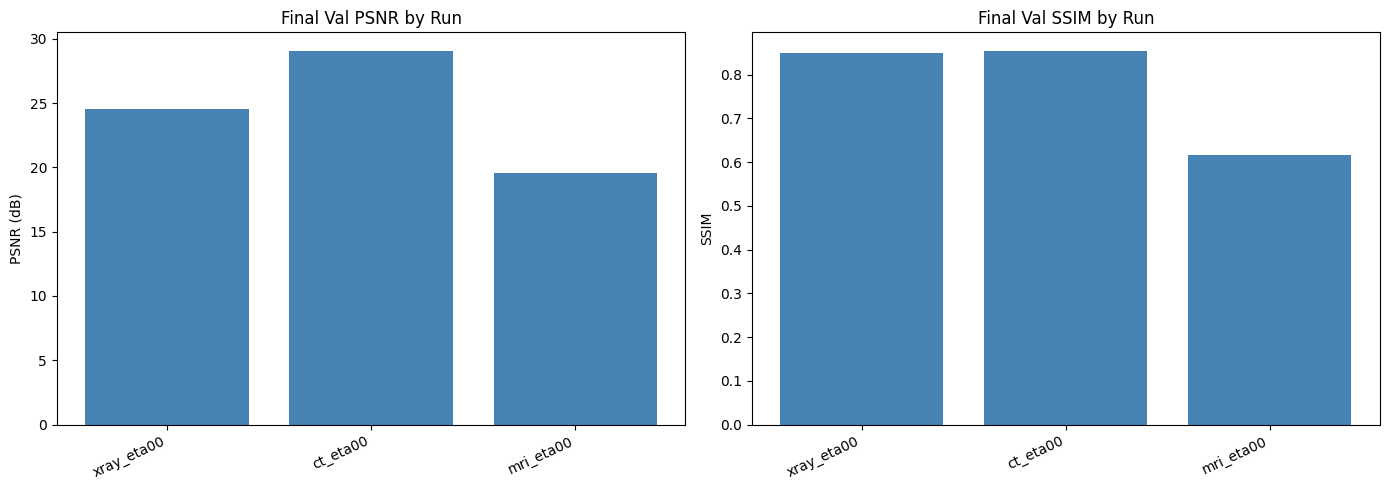
\includegraphics[width=\columnwidth]{figures/baseline_comparison.png}
  \caption{%
    Baseline PSNR (left) and SSIM (right) for all three modalities.
    CT benefits most from the edge representation; MRI suffers from
    information loss in soft-tissue edge maps.%
  }
  \label{fig:baseline_comparison}
\end{figure}

\subsection{SSD Results}

Table~\ref{tab:ssd} compares baseline and SSD performance at $\eta=0.8$.

\begin{table}[h]
\centering
\caption{Baseline vs.\ SSD ($\eta=0.8$) at epoch 50.
$\Delta$ columns show SSD minus baseline.}
\label{tab:ssd}
\small
\begin{tabular}{lcccccc}
\toprule
 & \multicolumn{2}{c}{PSNR (dB)} & \multicolumn{2}{c}{SSIM} \\
\cmidrule(lr){2-3}\cmidrule(lr){4-5}
Modality & Base & SSD & $\Delta$ & Base & SSD & $\Delta$ \\
\midrule
X-ray & 24.53 & 23.61 & $-0.92$ & 0.849 & 0.843 & $-0.006$ \\
CT    & 29.04 & 28.60 & $-0.44$ & 0.854 & 0.845 & $-0.009$ \\
MRI   & 19.57 & 19.66 & $+0.09$ & 0.616 & 0.595 & $-0.021$ \\
\bottomrule
\end{tabular}
\end{table}

Sparse supervision marginally degrades X-ray ($-0.92$\,dB) and CT
($-0.44$\,dB) reconstruction and has an essentially negligible effect on MRI
($+0.09$\,dB PSNR, $-0.021$ SSIM).
No modality benefits from the masking strategy.

Figure~\ref{fig:ssd_comparison} contrasts PSNR and SSIM across all six runs,
and Figure~\ref{fig:all_curves} overlays the learning curves for both
experiments.

\begin{figure}[h]
  \centering
  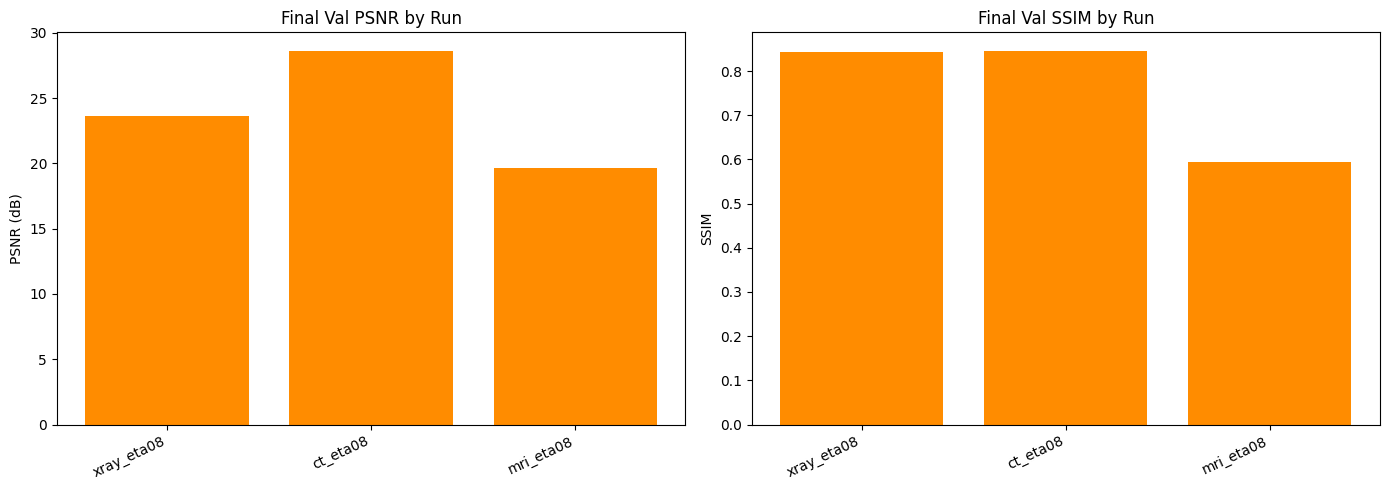
\includegraphics[width=\columnwidth]{figures/ssd_comparison.png}
  \caption{%
    PSNR (left) and SSIM (right) for SSD ($\eta=0.8$) runs.
    Performance is lower than or equal to the baseline across all modalities.%
  }
  \label{fig:ssd_comparison}
\end{figure}

% ── 6. Discussion ─────────────────────────────────────────────────────────────
\section{Discussion}
\label{sec:discussion}

\textbf{Why does SSD not help here?}
SSD was designed to prevent a generative model from memorising its small
training set by withholding pixel-level supervision \cite{ssd2025}.
In that setting, the model must hallucinate masked regions using global
structure, which strengthens the learned representation.
Our U-Net, however, does not exhibit memorisation: the validation loss tracks
the training loss closely in all baseline runs, and the model is initialised
from ImageNet-pretrained weights that already encode strong structural priors.
Masking 80\% of pixels per step therefore only reduces the effective amount of
supervision available without offering any compensating benefit---the
model already generalises well without the additional pressure.

\textbf{Modality ordering.}
The performance ranking (CT $>$ X-ray $>$ MRI) directly reflects the
information content preserved by edge operators.
CT produces high-contrast boundaries even at fine anatomical detail.
X-ray has strong Canny responses at lung and rib boundaries but more ambiguous
soft tissue.
MRI edges are sparse and weak; the model reconstructs coarse shape but not
intensity gradients within tissues.
Future work could explore modality-specific edge operators or learned feature
extractors to boost MRI performance.

\textbf{Scale of the experiment.}
Each model is trained on only 500 images for 50 epochs, which is a
deliberately compact regime.
With more data or longer training, both the baseline and SSD performances would
likely improve, and the relative ranking between the two loss regimes could
shift.

% ── 7. Conclusion ─────────────────────────────────────────────────────────────
\section{Conclusion}
\label{sec:conclusion}

We demonstrated that a pretrained ResNet34 U-Net can reconstruct medical images
from three-channel classical edge feature maps (Canny, Sobel, Laplacian) across
chest X-ray, chest CT, and brain MRI, achieving validation PSNR values of
24.5, 29.0, and 19.6\,dB respectively after 50 epochs on 500 training images
per modality.
A Sparsely Supervised Diffusion (SSD) masking loss with $\eta=0.8$ did not
improve reconstruction in any modality and modestly degraded CT and X-ray
quality, confirming that the memorisation problem SSD targets does not arise
with a well-regularised, pretrained regression network in this data regime.

% ── References ────────────────────────────────────────────────────────────────
\bibliographystyle{plain}
\begin{thebibliography}{9}

\bibitem{ssd2025}
Anonymous.
\newblock Sparsely Supervised Diffusion.
\newblock \textit{arXiv:2602.02699}, 2025.

\bibitem{unet2015}
O.~Ronneberger, P.~Fischer, and T.~Brox.
\newblock {U-Net}: Convolutional Networks for Biomedical Image Segmentation.
\newblock In \textit{MICCAI}, 2015.

\bibitem{he2016}
K.~He, X.~Zhang, S.~Ren, and J.~Sun.
\newblock Deep Residual Learning for Image Recognition.
\newblock In \textit{CVPR}, 2016.

\bibitem{canny1986}
J.~Canny.
\newblock A Computational Approach to Edge Detection.
\newblock \textit{IEEE Transactions on Pattern Analysis and Machine Intelligence},
  8(6):679--698, 1986.

\bibitem{adam2014}
D.~P. Kingma and J.~Ba.
\newblock Adam: A Method for Stochastic Optimization.
\newblock \textit{arXiv:1412.6980}, 2014.

\bibitem{imagenet2009}
J.~Deng, W.~Dong, R.~Socher, L.-J. Li, K.~Li, and L.~Fei-Fei.
\newblock {ImageNet}: A Large-Scale Hierarchical Image Database.
\newblock In \textit{CVPR}, 2009.

\bibitem{xray_data}
M.~E.~H.~Chowdhury et~al.
\newblock {COVID-19 Radiography Database}.
\newblock \url{https://www.kaggle.com/datasets/tawsifurrahman/covid19-radiography-database}, 2020.

\bibitem{ct_data}
M.~Hany.
\newblock Chest {CT} Scan Images.
\newblock \url{https://www.kaggle.com/datasets/mohamedhanyyy/chest-ctscan-images}, 2020.

\bibitem{mri_data}
N.~Patel.
\newblock Brain {MRI} Images for Brain Tumor Detection.
\newblock \url{https://www.kaggle.com/datasets/navoneel/brain-mri-images-for-brain-tumor-detection}, 2019.

\end{thebibliography}

% ── Appendix: Reconstruction Grids and Curves ─────────────────────────────────
\appendix
\onecolumn

\section{Reconstruction Grids}
\label{app:grids}

Each row in the grids below shows five columns:
\textbf{Canny edge map} $|$ \textbf{Sobel gradient magnitude} $|$
\textbf{Laplacian} $|$ \textbf{Model prediction} $|$ \textbf{Ground truth}.

\begin{figure}[H]
  \centering
  \begin{subfigure}{\textwidth}
    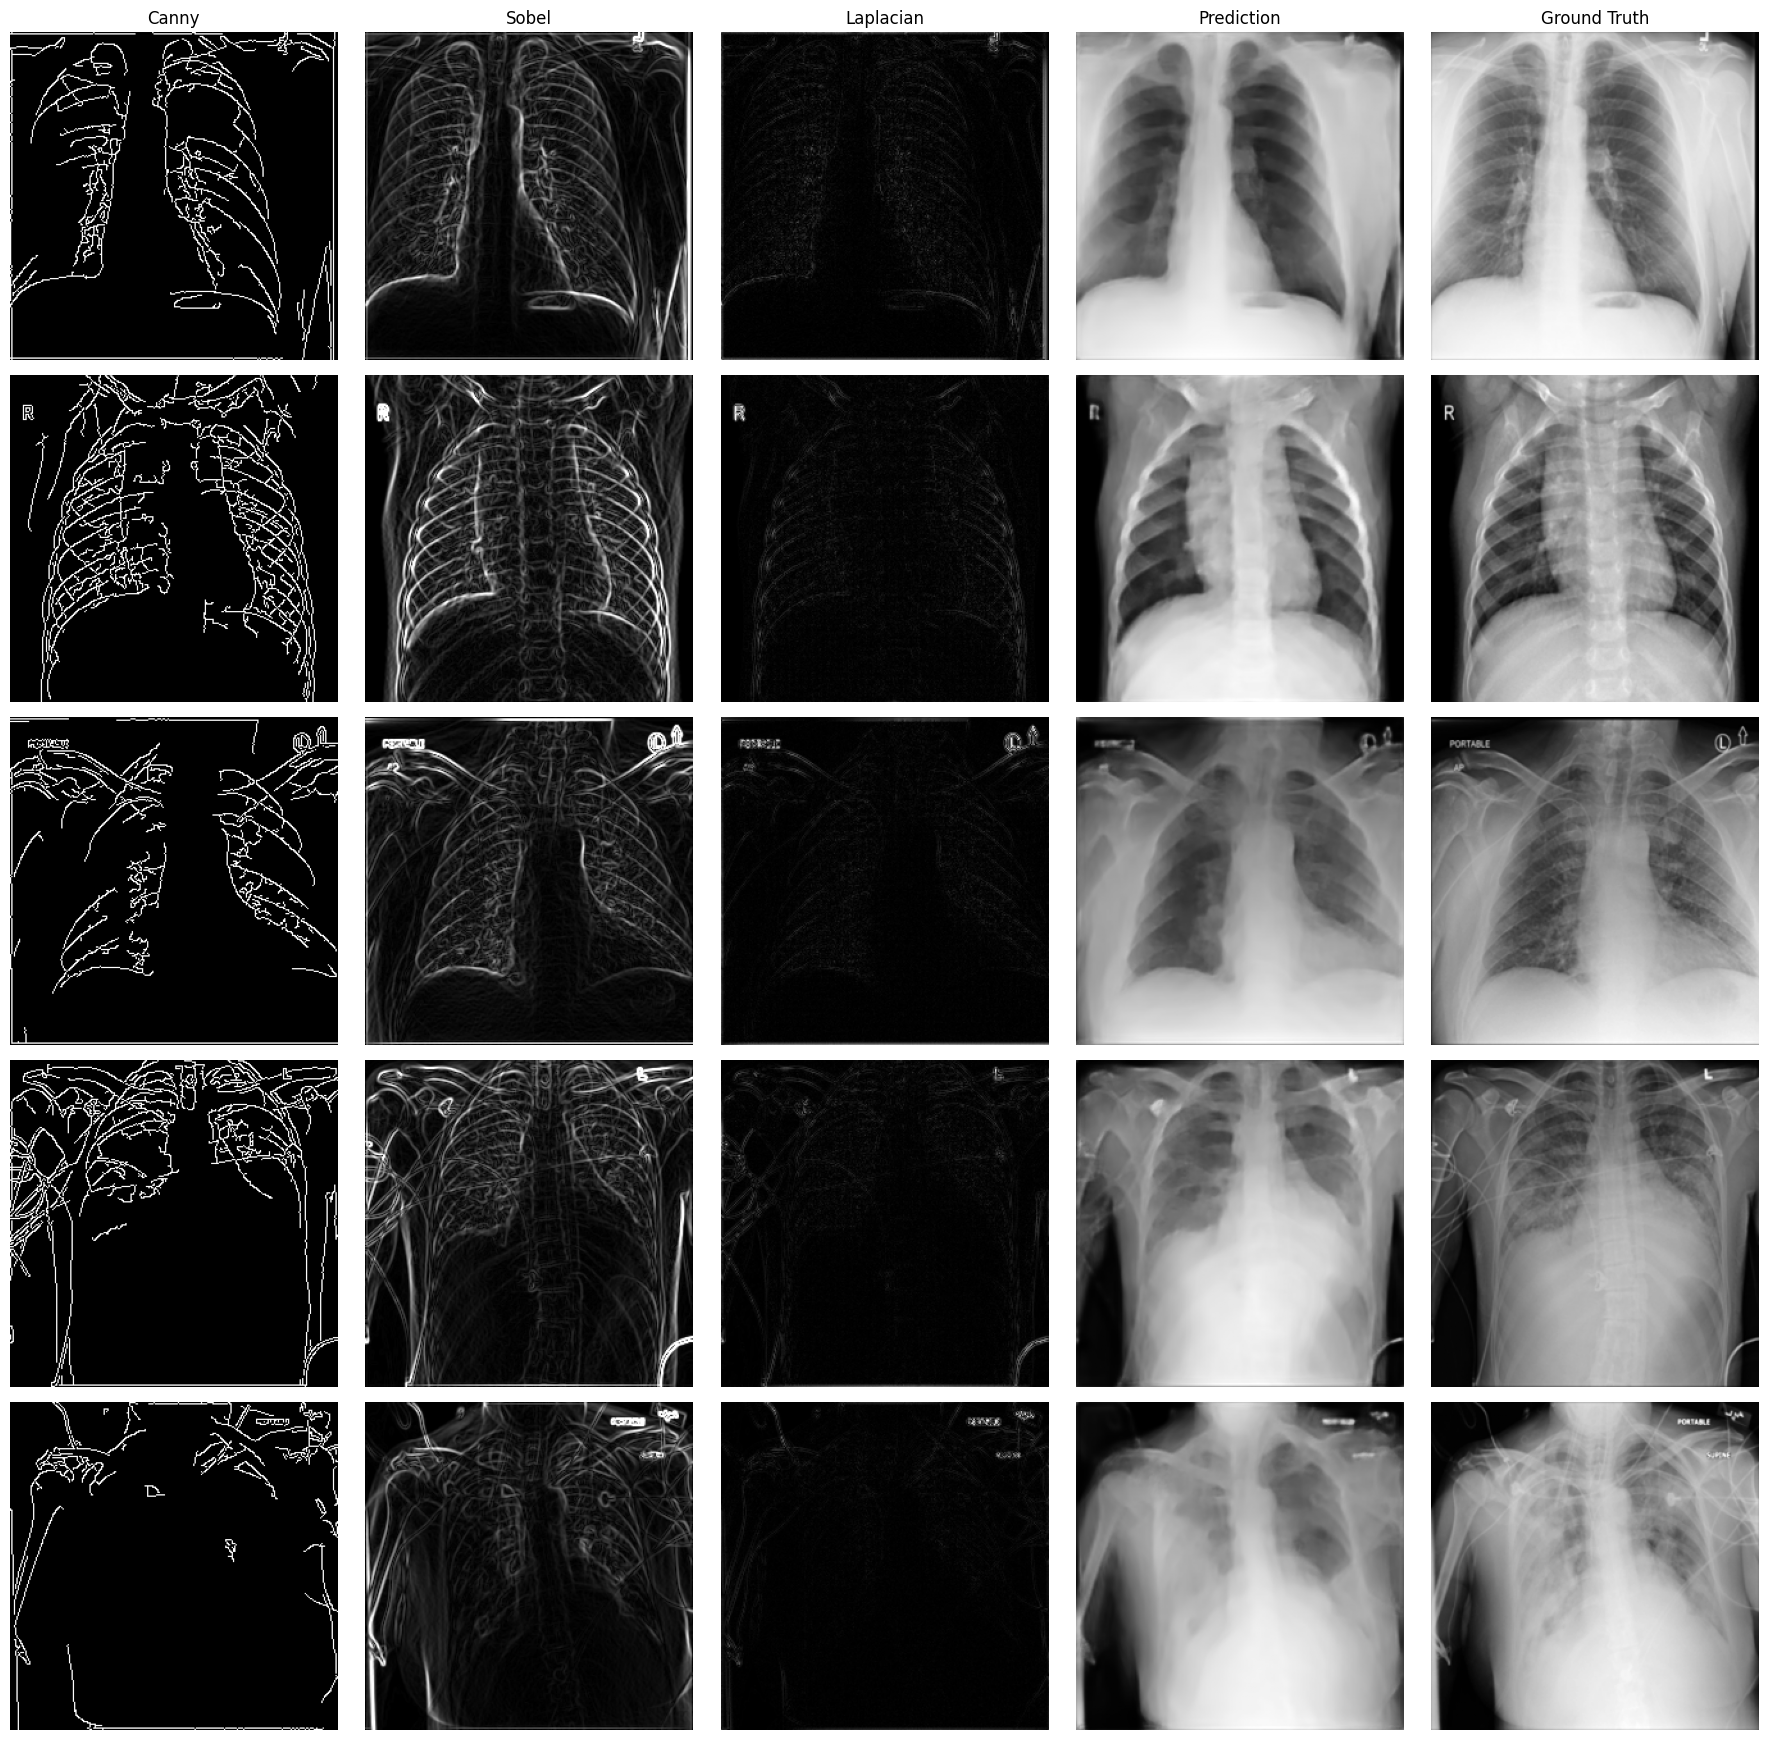
\includegraphics[width=\textwidth]{figures/xray_baseline_grid.png}
    \caption{X-ray baseline ($\eta=0$). Global anatomy (lung fields, ribs,
    mediastinum) is well-recovered; fine texture is smoothed.}
  \end{subfigure}
  \vspace{0.5em}
  \begin{subfigure}{\textwidth}
    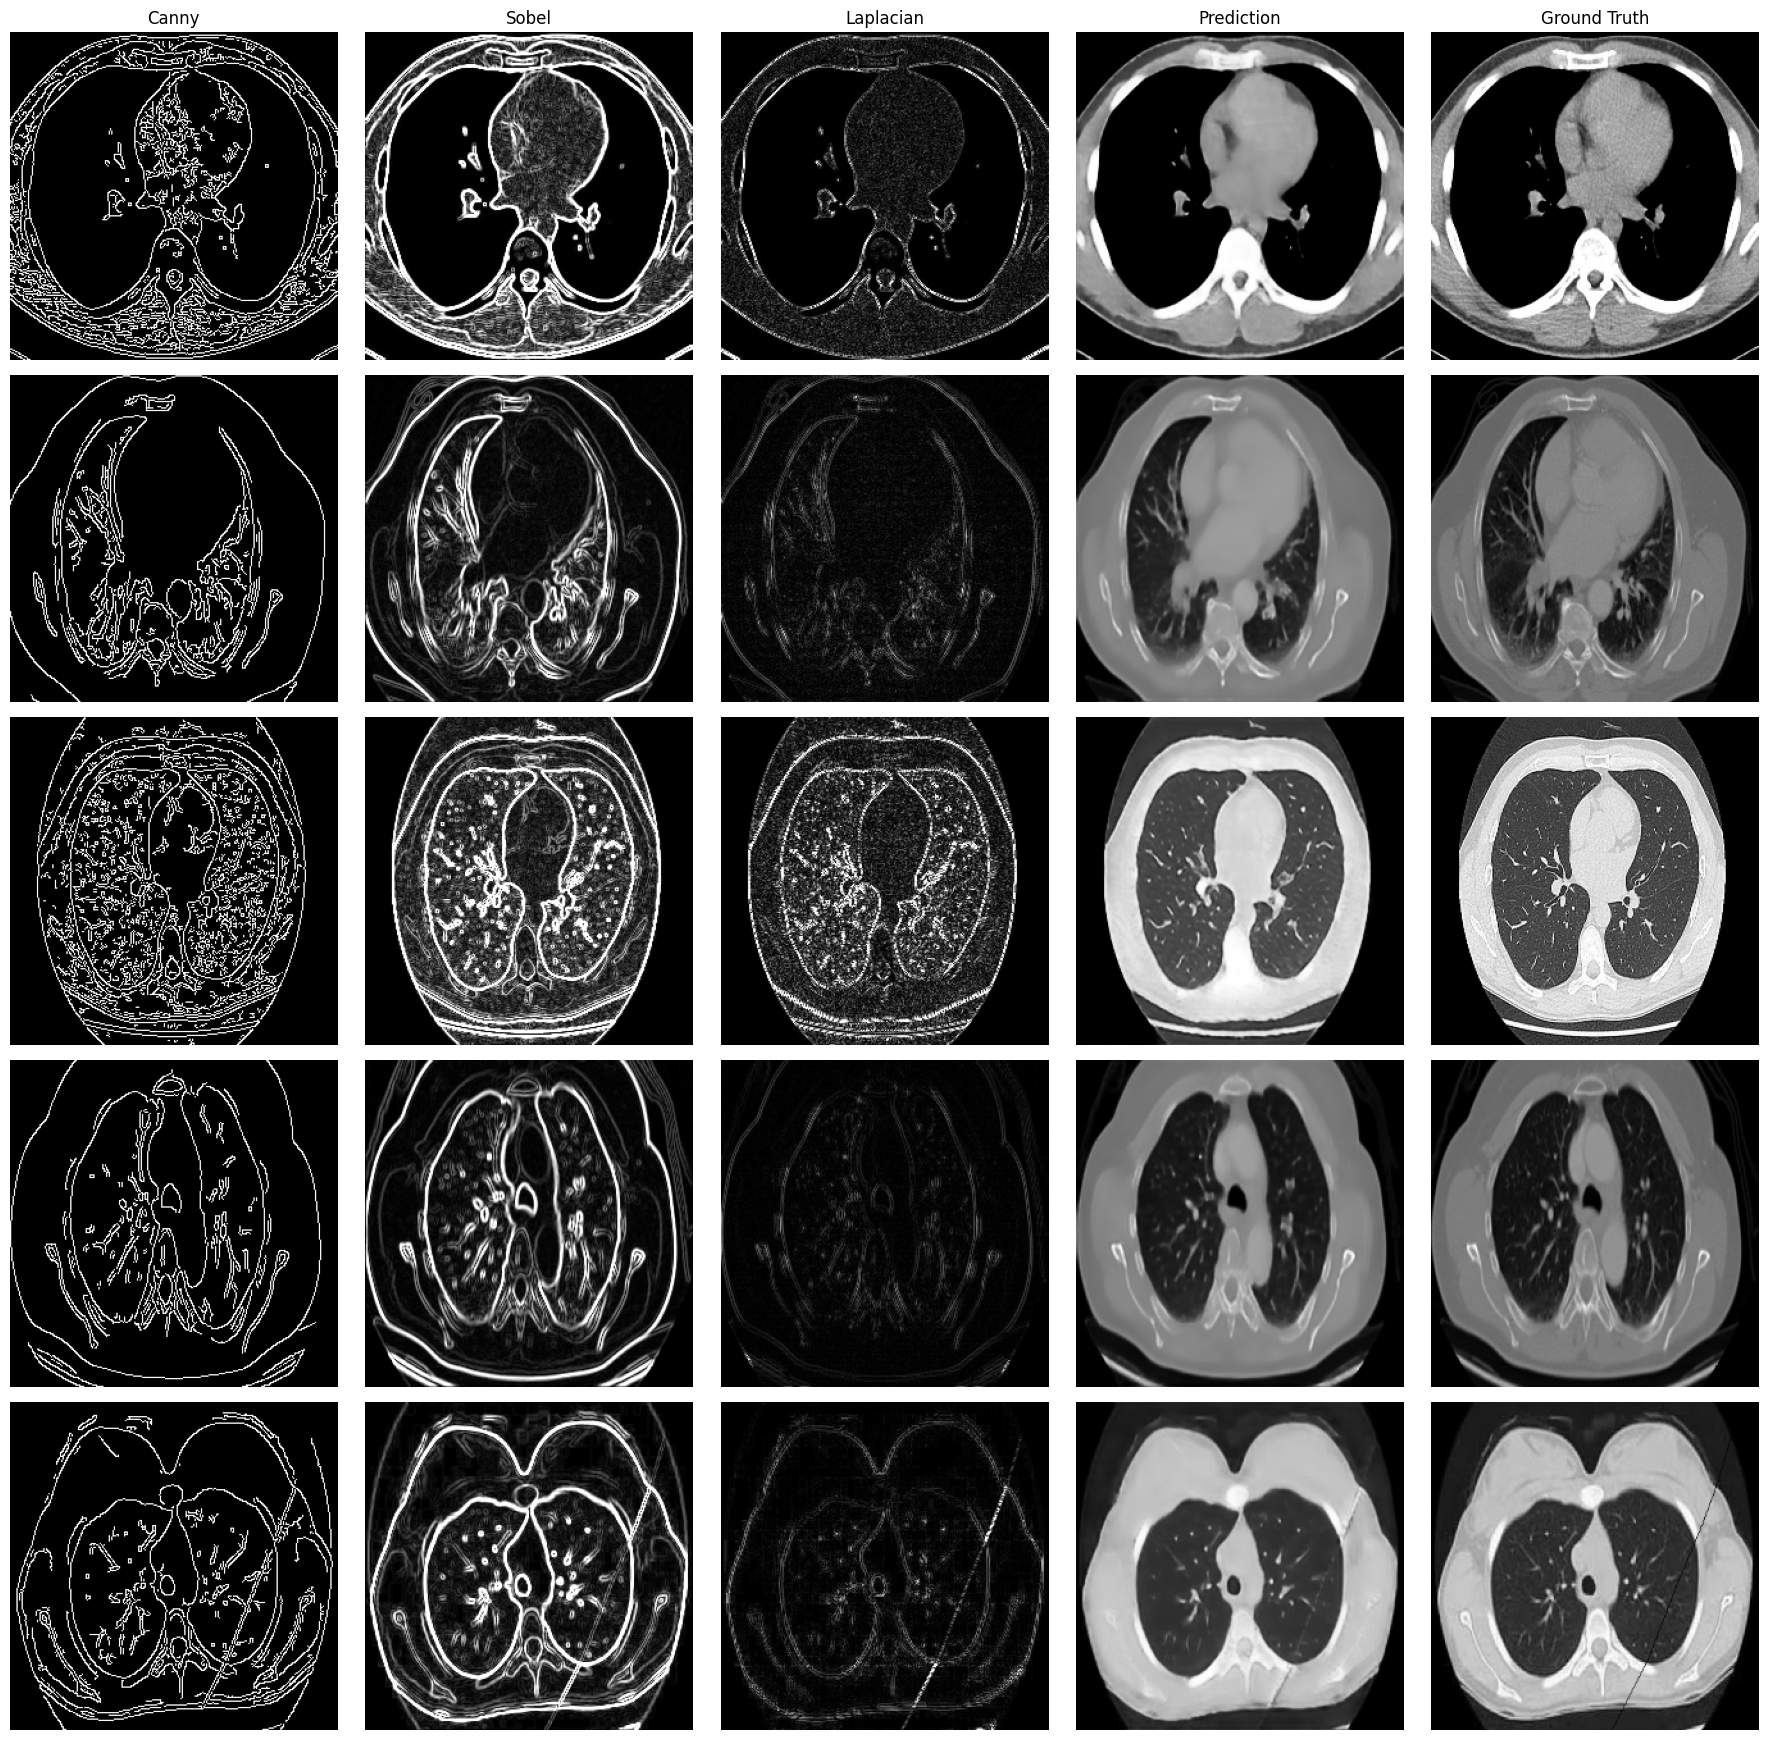
\includegraphics[width=\textwidth]{figures/ct_baseline_grid.png}
    \caption{CT baseline ($\eta=0$). Predictions are nearly indistinguishable
    from ground truth; sharp tissue interfaces are faithfully reconstructed.}
  \end{subfigure}
  \vspace{0.5em}
  \begin{subfigure}{\textwidth}
    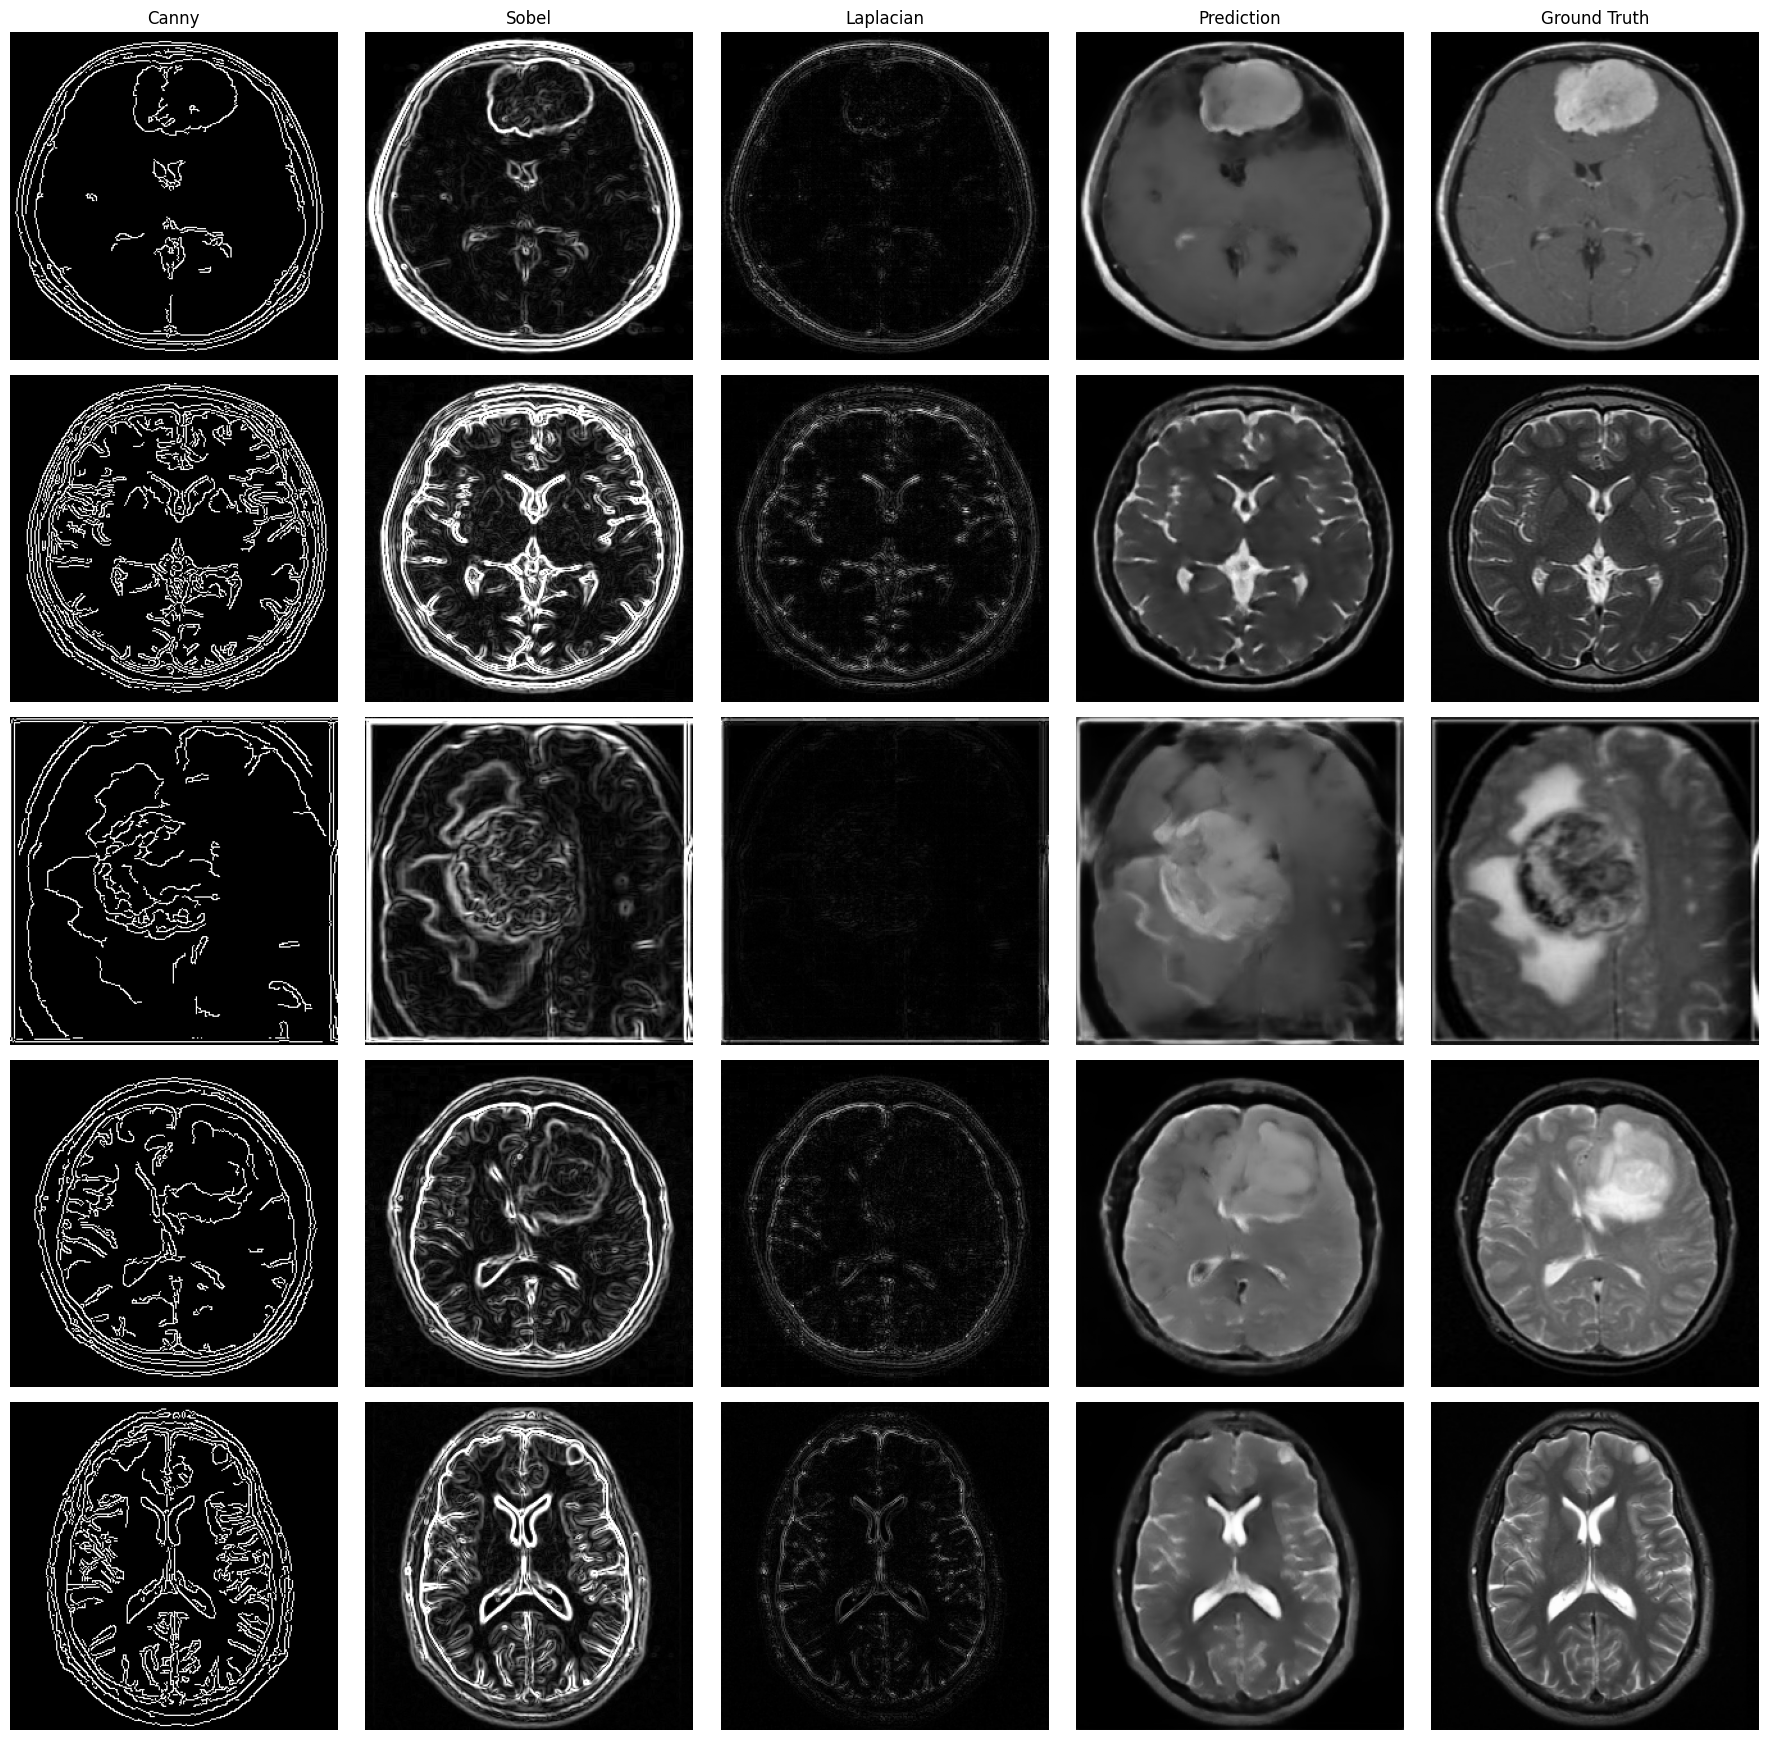
\includegraphics[width=\textwidth]{figures/mri_baseline_grid.png}
    \caption{MRI baseline ($\eta=0$). Coarse head shape is recovered but
    internal soft-tissue contrast and tumour regions are blurred.}
  \end{subfigure}
  \caption{Baseline reconstruction grids for all three modalities.}
  \label{fig:grids_baseline}
\end{figure}

\begin{figure}[H]
  \centering
  \begin{subfigure}{\textwidth}
    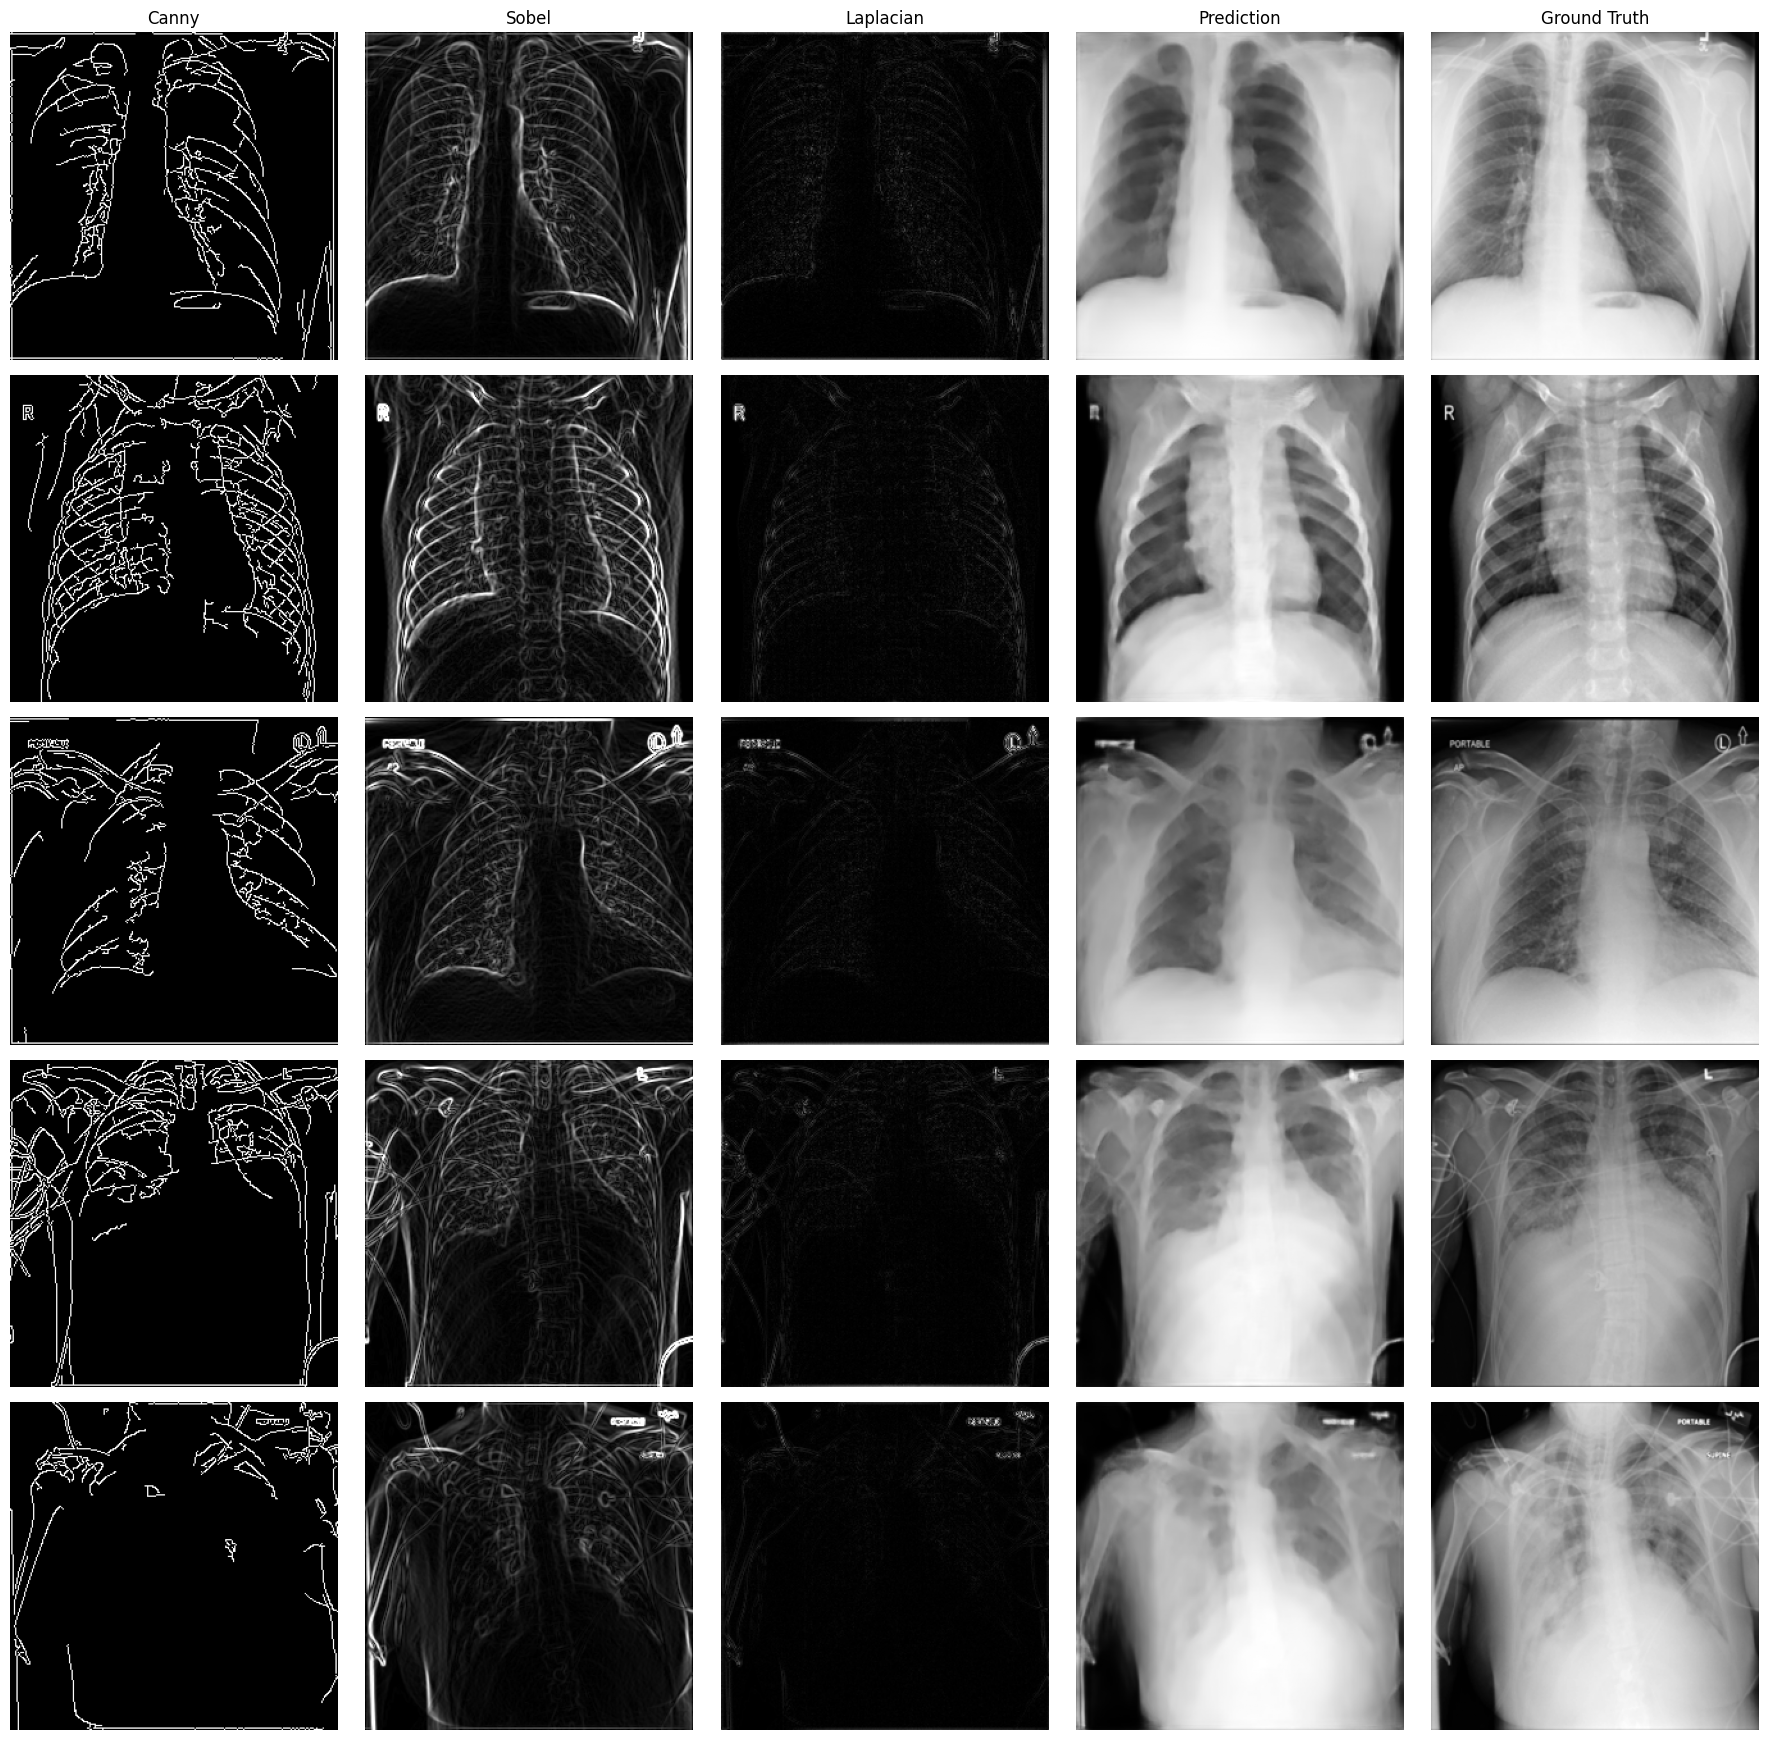
\includegraphics[width=\textwidth]{figures/xray_ssd_grid.png}
    \caption{X-ray SSD ($\eta=0.8$).}
  \end{subfigure}
  \vspace{0.5em}
  \begin{subfigure}{\textwidth}
    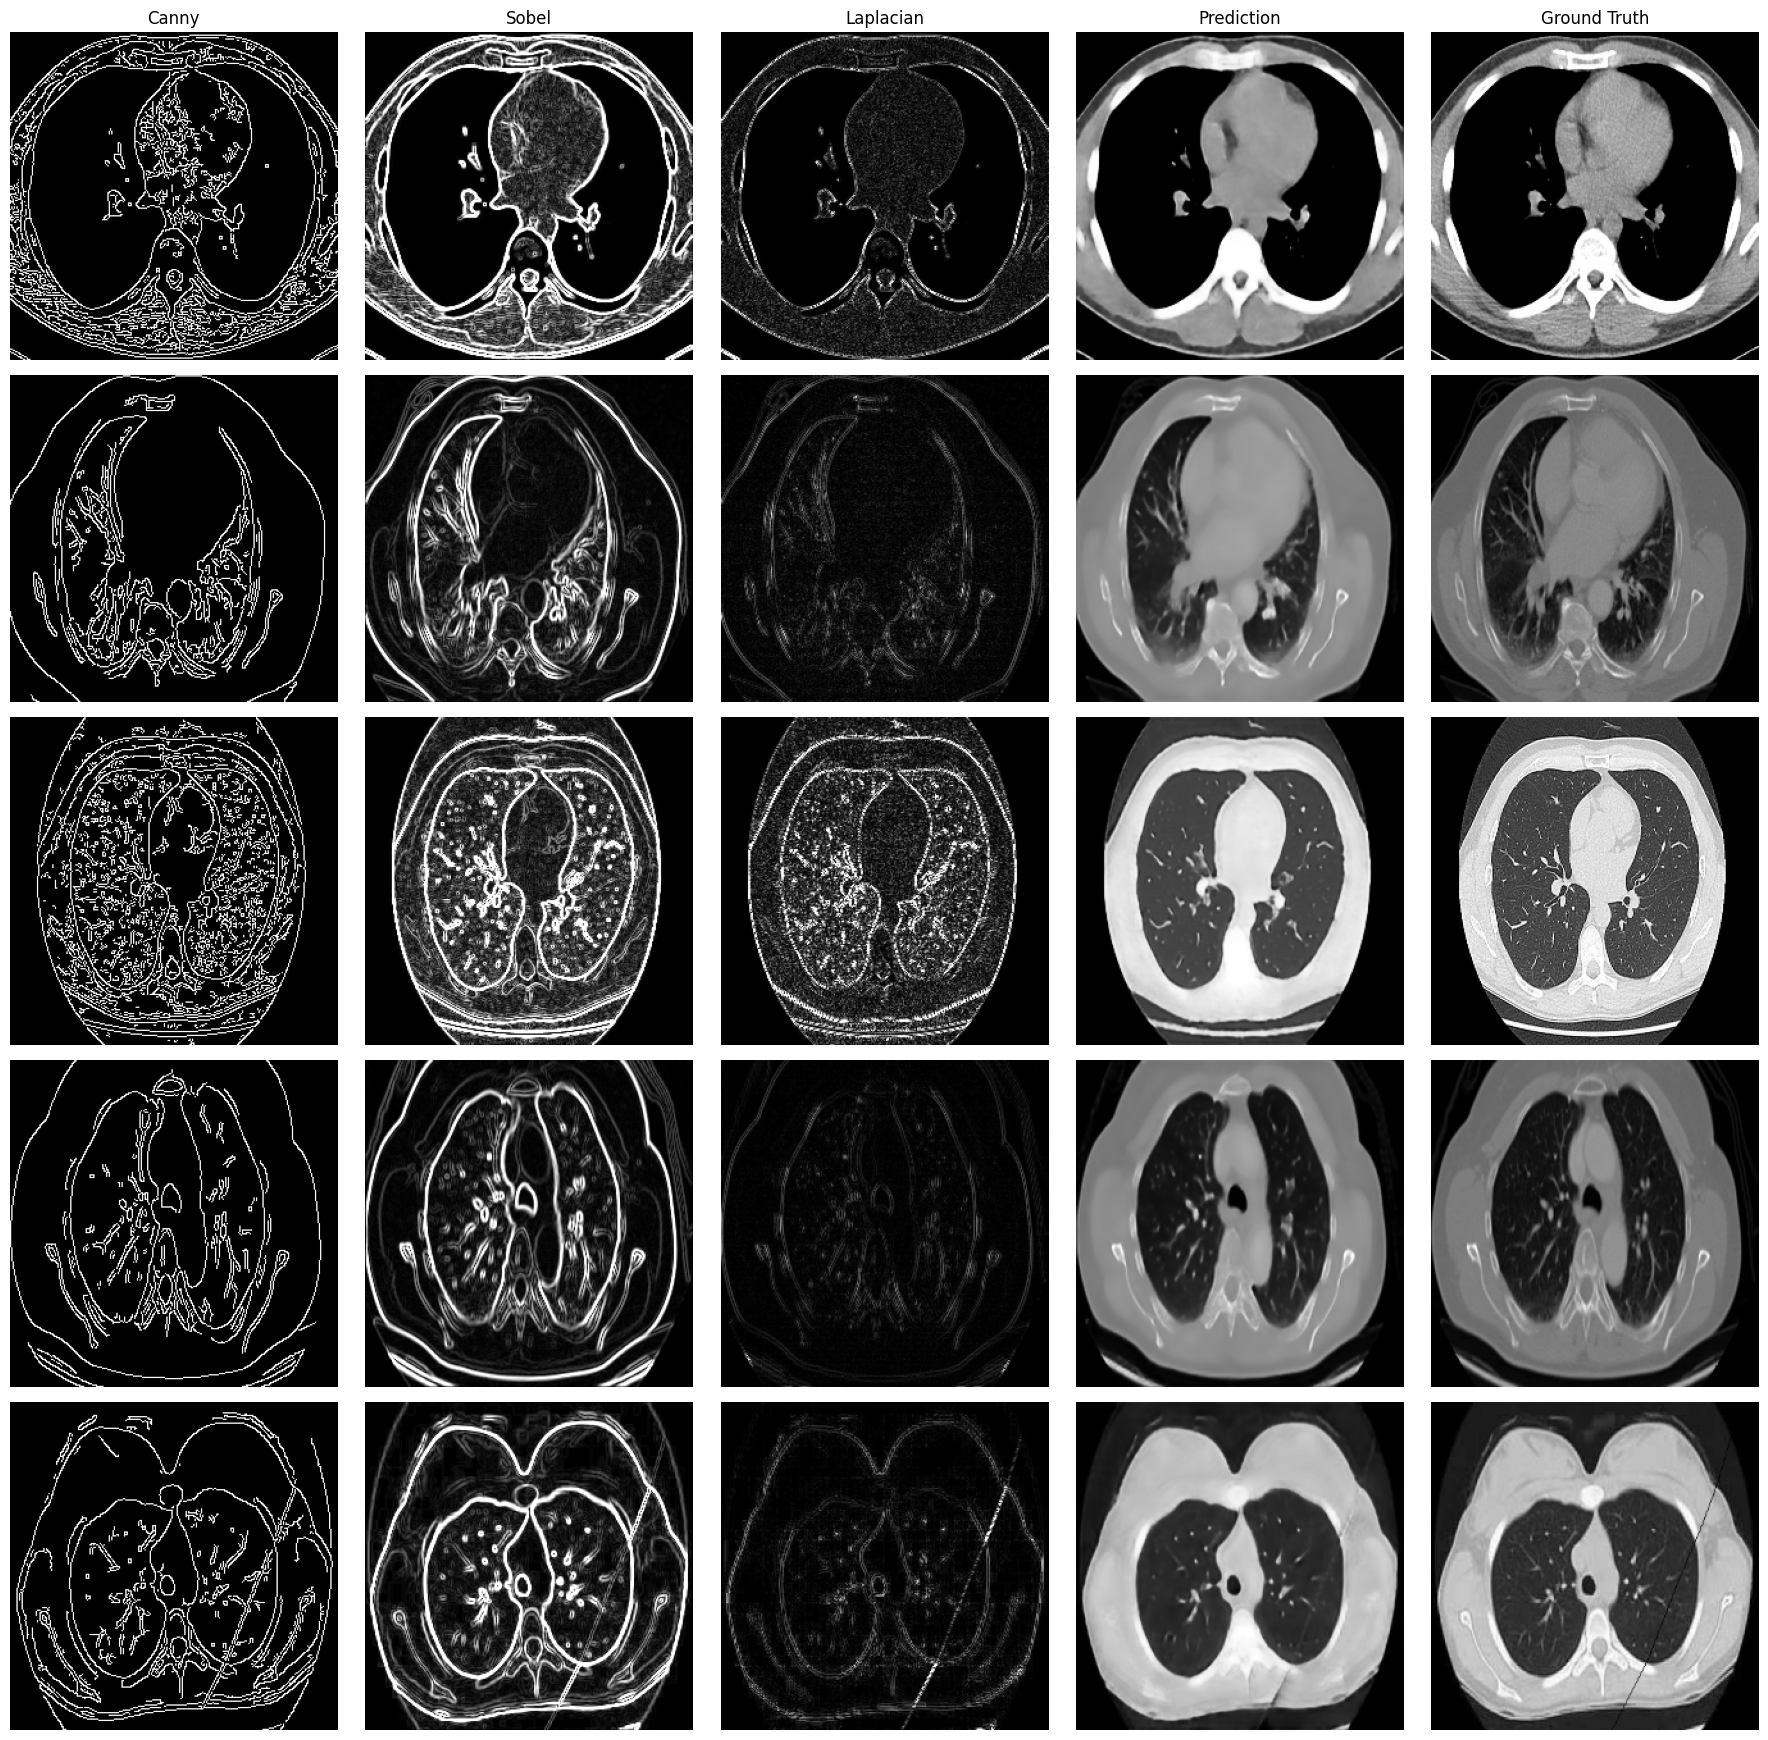
\includegraphics[width=\textwidth]{figures/ct_ssd_grid.png}
    \caption{CT SSD ($\eta=0.8$).}
  \end{subfigure}
  \vspace{0.5em}
  \begin{subfigure}{\textwidth}
    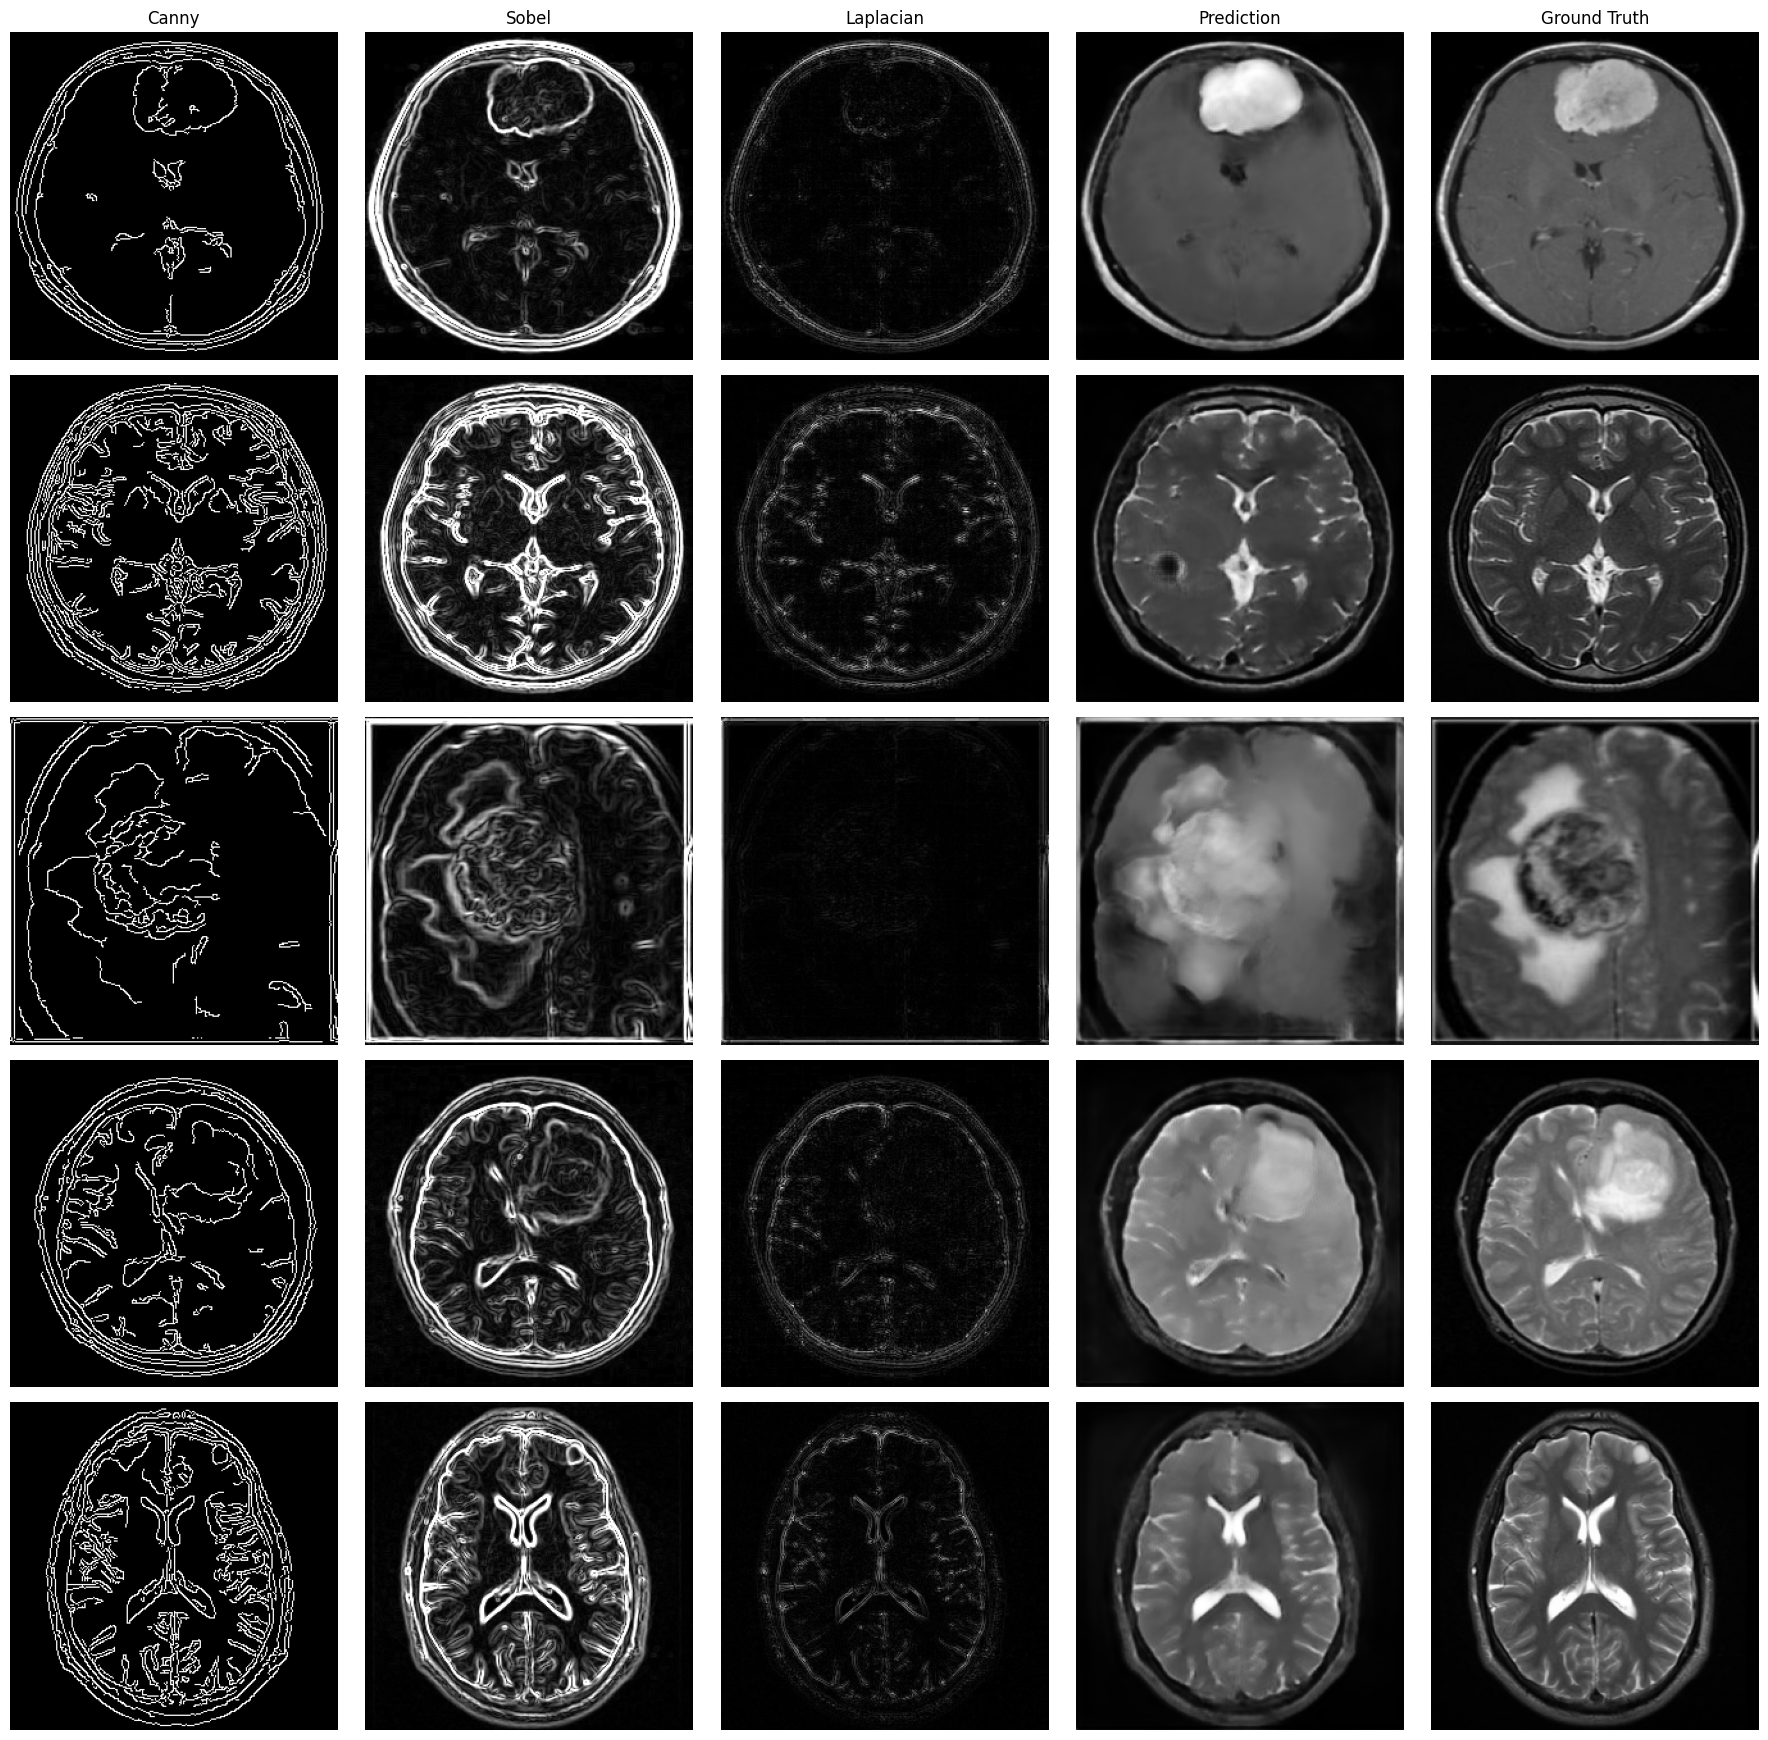
\includegraphics[width=\textwidth]{figures/mri_ssd_grid.png}
    \caption{MRI SSD ($\eta=0.8$).}
  \end{subfigure}
  \caption{SSD ($\eta=0.8$) reconstruction grids. Visual quality is comparable
    to baseline; quantitative metrics show a small degradation for X-ray and CT.}
  \label{fig:grids_ssd}
\end{figure}

\section{Training and Validation Curves}
\label{app:curves}

\begin{figure}[H]
  \centering
  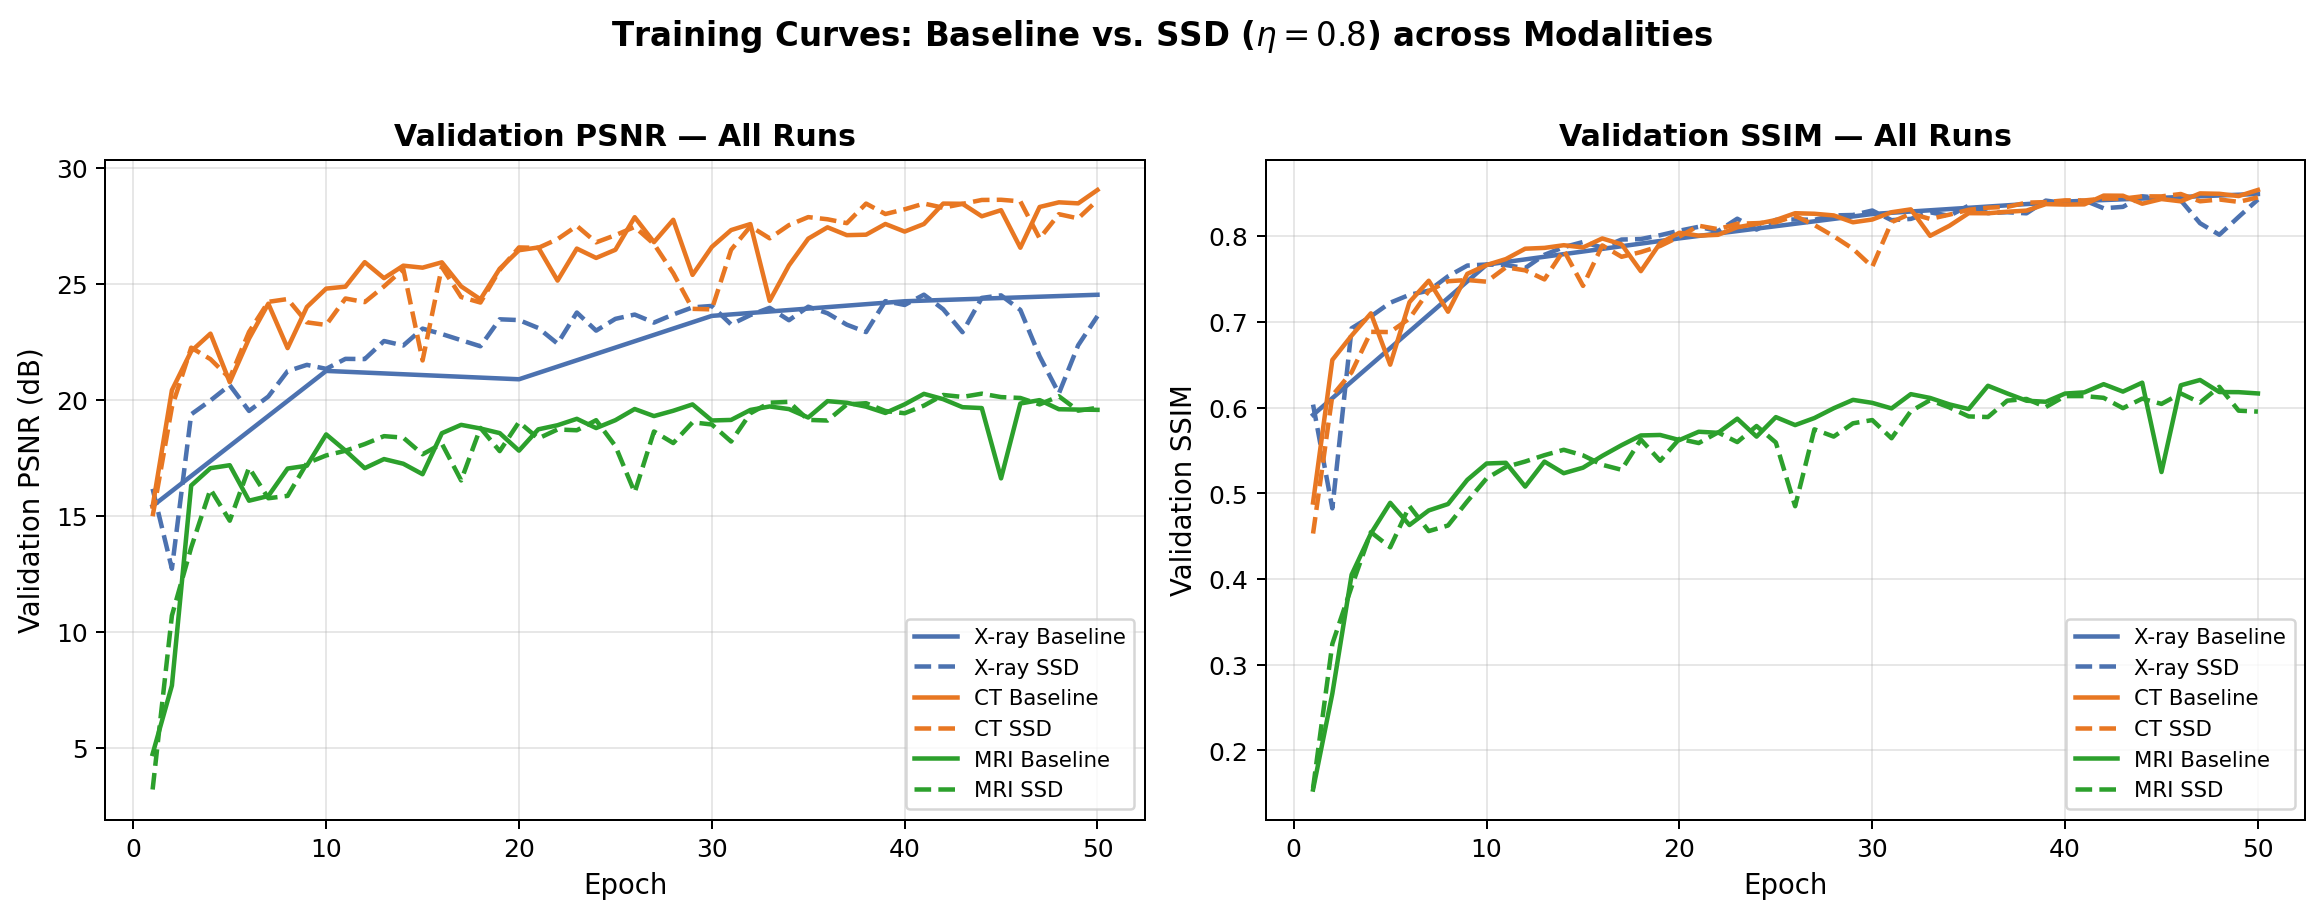
\includegraphics[width=0.85\textwidth]{figures/all_curves.png}
  \caption{%
    Validation PSNR (left) and SSIM (right) over 50 training epochs for all
    six models. Solid lines are baseline runs; dashed lines are SSD ($\eta=0.8$)
    runs. Both metrics improve rapidly in the first 10--15 epochs and plateau
    thereafter. The baseline consistently meets or exceeds the SSD variant.%
  }
  \label{fig:all_curves}
\end{figure}

\begin{figure}[H]
  \centering
  \begin{subfigure}{0.32\textwidth}
    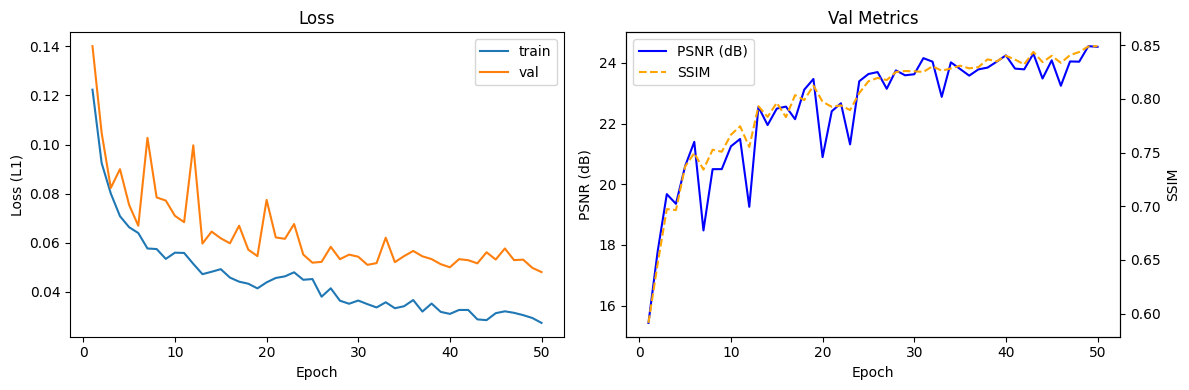
\includegraphics[width=\textwidth]{figures/xray_curves.png}
    \caption{X-ray baseline}
  \end{subfigure}
  \hfill
  \begin{subfigure}{0.32\textwidth}
    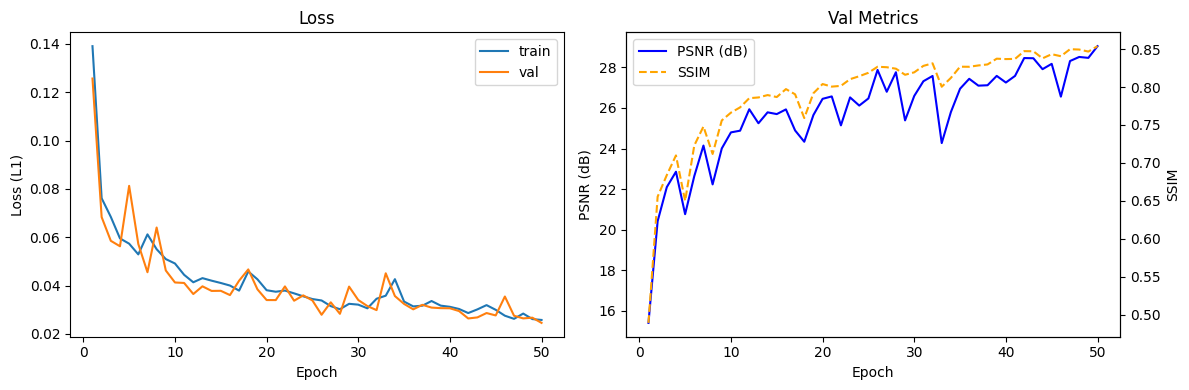
\includegraphics[width=\textwidth]{figures/ct_curves.png}
    \caption{CT baseline}
  \end{subfigure}
  \hfill
  \begin{subfigure}{0.32\textwidth}
    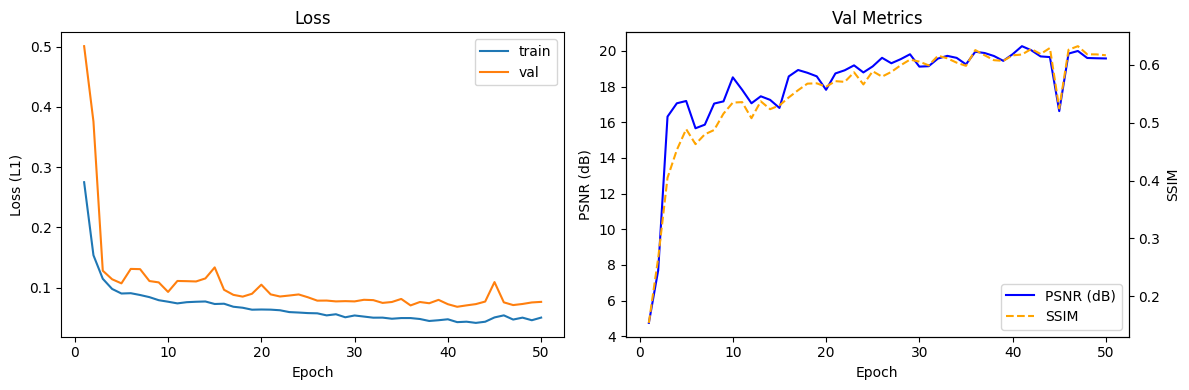
\includegraphics[width=\textwidth]{figures/mri_curves.png}
    \caption{MRI baseline}
  \end{subfigure}
  \caption{%
    Per-modality training curves for the baseline experiment.
    Each plot shows training loss (blue), validation loss (orange), PSNR, and
    SSIM over 50 epochs.
    CT converges fastest and achieves the lowest validation loss; MRI starts
    with high validation loss due to the sparse edge maps.%
  }
  \label{fig:curves}
\end{figure}

\end{document}
